\documentclass[fontsize=14pt,a4paper,headinclude,DIV=calc,automark]{scrbook}

\usepackage{float}
\usepackage[left=3cm,right=2cm,top=2.5cm,bottom=2.5cm]{geometry} % Seitenränder
\usepackage{polyglossia}
\setmainlanguage{german}
\setotherlanguage{english}
\hyphenation{Kran-ken-hau-ses Pro-dukt-de-signer Be-rufs-bil-dungs-werk}

\usepackage[
    format=plain,
    labelformat=empty,
    textfont={small,it,singlespacing},
   %justification=raggedright,
    belowskip=-6pt
 ]{caption}

\usepackage{setspace}       % Für Zeilenabstand
\usepackage{booktabs}       % Für professionelle Tabellenlinien
\usepackage{eurosym}        % Für das Euro-Symbol
\usepackage{graphicx}       % Für das Einbinden von Grafiken
\usepackage{fancybox}       % Für Rahmen um Text und Bilder
\usepackage{mdframed}       % Für Rahmen um Text und Bilder

\usepackage[
    colorlinks=true,
    urlcolor=blue,
    linkcolor=green
]{hyperref}    

\usepackage{scrlayer-scrpage} % Paket einfach laden, Optionen zentral setzen
\KOMAoptions{
    automark,             % Wichtig: Aktiviert die automatische Markierung
    markcase=nouppercase, % Verhindert Großbuchstaben in den Kopfzeilen
    headsepline=0.4pt,    % Linie unter der Kopfzeile
    footsepline=0pt,      % Keine Linie über der Fußzeile
    chapterprefix=true    % Auch wenn Kapitel nicht nummeriert sind, oft hilfreich
}

\RedeclareSectionCommand[
  runin=false,
  afterindent=false,
  beforeskip=.5\baselineskip,
  afterskip=5pt]{section}

\raggedbottom

%\rohead{\leftmark} % Unkommentieren, falls die Seitenzahlen in der Fußzeile erscheinen sollen

\setkomafont{pageheadfoot}{\color{myblue}} % Stellt sicher, dass die Schriftart der Kopf-/Fußzeile neutral ist

\usepackage[dvipsnames]{xcolor}
\definecolor{myblue}{RGB}{47, 84, 150}
\definecolor{rahmenlinie}{RGB}{127, 127, 127}

\usepackage{fontspec}
%\setmainfont{Palatino Linotype}
%\setsansfont{Palatino Linotype}
%\setmonofont{Palatino Linotype}
\setmainfont{Cambria}
\setsansfont{Calibri}
\setmonofont{Calibri}

\setkomafont{chapter}{\normalfont\huge\rmfamily\textcolor{myblue}}
\setkomafont{section}{\normalfont\fontsize{18}{24}\rmfamily\textcolor{myblue}}
\setkomafont{subsection}{\normalfont\large\rmfamily\textcolor{myblue}}

\linespread{1.2}

\setcounter{secnumdepth}{-1} % Deaktiviert die Nummerierung für alle Überschriften

\title{Mitleid? Nein, danke!}
\author{Marius Ebel}
\date{November 2024}

\clubpenalty=10000    % Verhindert Schusterjungen (erste Zeile eines Absatzes am Seitenende)
\widowpenalty=10000   % Verhindert Hurenkinder (letzte Zeile eines Absatzes am Seitenanfang)


\begin{document}
\frontmatter



\thispagestyle{empty}
\vspace*{\fill}
\begin{center}
    \huge\bfseries Mitleid? - Nein, danke!\par
    \vspace{1cm}
    \large Meine Geschichte: Ein Leben mit Freude trotz\\ unheilbarer Krankheit\par
    \vspace{1cm}
    \normalsize von \textit{Marius Ebel}\par
\end{center}
\vspace*{\fill}

\pagestyle{plain}
\addchap{Danksagung}
\addcontentsline{toc}{chapter}{Danksagung}

Ich möchte mich bei all jenen bedanken, die mich dabei unterstützt haben, diese Autobiographie zu schreiben und die mich dazu ermuntert haben, am Ball zu bleiben, wenn Zweifel in mir aufkamen.
Ein besonderer Dank gilt dabei Anja Schulte, Roland Penz und Rüdiger Barth vom Kinder- und Jugendhospiz Balthasar, die mir dieses Projekt ans Herz gelegt haben, und ebenso Rebecca Kranz, die die Organisation übernommen und dafür gesorgt hat, dass aus dem Text ein richtiges Buch geworden ist.

Danksagen möchte ich auch allen Mitarbeiter:innen des Balthasars. Danke für eure Verbundenheit, eure Fürsorge und Gastfreundschaft. Ihr seid es, die das Balthasar für mich zu einem zweiten Zuhause haben werden lassen.
Ebenso bedanken möchte ich mich bei allen, die mich bei diesem Projekt in der ein oder anderen Form unterstützt haben. Ohne ihre Hilfe wäre dieses Buch nicht möglich gewesen.

Schließlich will ich an dieser Stelle auch meine Eltern erwähnen, deren Liebe ich mir ebenso sicher sein kann wie ihrer Unterstützung, wann immer ich sie brauche. Ihr wart und seid immer für mich da und ermutigt mich, meinen eigenen Weg zu gehen. Ihr habt mir gezeigt, dass das Leben trotz aller Herausforderungen lebenswert ist und dass es sich lohnt, für seine Träume zu kämpfen.

\vspace{0.5cm}
\noindent\textit{Marius Ebel}

\addchap{Statt eines Vorwortes}
\addcontentsline{toc}{chapter}{Statt eines Vorwortes}
Lieber Marius,\par
\vspace*{0.5\baselineskip}
\noindent als ich in Deinem Alter war, hatte ich mir auch gerade einen Traum erfüllt: Ich war in meinem ersten Theaterengagement.
Der Weg dorthin war eher alptraumhaft. Ich hatte kaum Kohle für Fahrten und Bewerbungen. Ich hatte an allen Schauspielschulen Aufnahmeprüfungen abgelegt und alle versicherten mir, dass es mir an Talent fehlt. Ich hatte einen Minderwertigkeitskomplex, der für mehrere Leben gereicht hätte.
Aber ich wollte, nein, musste doch Schauspieler werden.

Zunächst parkte ich mich auf der Bank. Einer großen deutschen Bank, die mich ausbildete. Mein kreatives Potenzial konnte ich dort nicht gerade ausleben. Eher lernte ich dort, wie man einen Lederschlips bindet, man ab 15 Uhr nicht mehr ans Telefon geht und man Greisen Sparpläne über 20 Jahre aufdrückt. (Alles Dinge, die mir für bestimmte Rollen später wichtig sein sollten, das wusste ich damals aber noch nicht…)

Allen Absagen und Unkenrufen zum Trotz hielt ich an meinen Versuchen fest, meinen Traum zu verwirklichen.
Ich ließ nicht locker und zog mich an meinem – damals noch vorhandenen – Haarschopf aus dem einen oder anderen Loch. Mein Langmut, meine Beharrlichkeit und mein Selbstverwirklichungsdrang setzten sich am Ende durch, und mittlerweile bin ich dankbar für die gemachten Erfahrungen.

Auf gewisse Weise erinnerst Du, Marius, mich an mich. Nicht nur, dass Dein Name die männliche Variante meines zweiten Vornamens ist, strebst Du auch danach, Dich auszudrücken, kreativ zu sein, der Welt etwas zu schenken. Und dieses Geschenk, das gleichsam Dein Vermächtnis ist, halten wir nun in den Händen.
Danke dafür. Danke, dass Du uns an Dir teilhaben lässt. Danke, dass Du diesen Kraftakt vollzogen hast.
Ein schlauer Mensch hat mal gesagt: Es ist schön, wenn man tun kann, was man will. Es ist schöner, wenn man tun will, was man kann.
Du kannst. Und wie!

Schenk uns weitere Bücher. Ich weiß schon jemanden, der gerne wieder ein Vorwort schreiben wird, das keins ist…

\vspace{0.5cm}
\noindent\textit{Dein Christoph Maria Herbst}

\begin{figure}[ht] % [htbp] sind Platzierungsoptionen: h=here, t=top, b=bottom, p=page
    \centering % Zentriert die Abbildung auf der Seite
    \includegraphics[width=0.8\textwidth]{Fotos/ChristophMariaHerbst.jpg}
    \label{fig:ChristophMariaHerbst} % Label für Querverweise
\end{figure}

\addchap{Warum es dieses Buch gibt}
\addcontentsline{toc}{chapter}{Warum es dieses Buch gibt}

\textit{„Wie kommst Du damit klar?“}, fragte mich die Frau ganz direkt. Wir hatten bereits eine Zeit lang über dies und das geplaudert. Gemeinsam mit der pädagogischen Leiterin der Einrichtung saßen wir im Leseraum des Kinder- und Jugendhospizes Olpe und ich überlegte, wie ich ihre Frage beantworten wollte. Es ging um die Krankheit, an der ich leide: eine fortschreitende Form von Muskelschwund. Die Antwort, die ich ihr dann gab, klingt vielleicht banal: \textit{„Man wächst einfach hinein.“} Und genauso ist es.

Das war 2020 während eines Aufenthalts im Balthasar. Ich war gerade angekommen. Meine Eltern hatten die Koffer ausgeräumt, meine Klamotten in den Schränken verstaut, Laptop und Playstation angeschlossen und sich nach der üblichen Abschiedszeremonie auf den Heimweg gemacht. Anja Schulte, die damalige pädagogische Leiterin, kam in mein Zimmer und fragte mich, ob ich Zeit und Lust auf ein Gespräch hätte. Die Mutter eines sechsjährigen Jungen, der ebenfalls mit Duchenne Muskeldystrophie auf die Welt gekommen war, wollte die Gelegenheit nutzen und sich mit jemandem austauschen, der an der gleichen Krankheit litt wie ihr Sohn. Jemand, der sozusagen aus erster Hand berichten und ihr Tipps geben konnte.
Natürlich hatte ich Zeit. Und Lust.

So trafen wir uns noch am gleichen Nachmittag. Die Frau war ziemlich taff; sie erinnerte mich an meine Mutter. In ihrem Sohn, der mir zuvor schon im Aufenthaltsbereich aufgefallen war, sah ich mich selbst vor über 20 Jahren. Ich beantwortete ihre Fragen so gut ich konnte, beispielsweise welche medizinischen Eingriffe ich hinter mir habe, warum ich mich für die eine oder andere Operation entschieden habe, welche Hilfsmittel ich in der Vergangenheit in Anspruch genommen habe und welche ich zurzeit nutze, aber auch wie meine Erfahrungen mit den Krankenkassen sind und welche Therapien ich mache.

Die Zeit flog nur so dahin. Obwohl das Gespräch über zwei Stunden dauerte, kam es mir vor wie zehn Minuten. Ich hoffe sehr, dass ich der Frau habe helfen können, indem ich ihr von meinem Leben mit der Krankheit erzählte und von meinen Erfahrungen, in der Kindheit, der Jugend, bis zum heutigen Tag. Vielleicht konnte ich ihr auch vor Augen führen, dass man als Mittzwanziger mit Duchenne durchaus zuversichtlich und lebensbejahend sein kann und nicht zurückgezogen und in sich gekehrt sein muss – was wohl viele denken – und dass die Krankheit das Leben der Betroffenen und ihrer Familien zwar in vielen Bereichen beherrscht, aber eben nicht komplett.

Für mich war das Gespräch mit dieser Mutter eine Bereicherung. Hört sich jetzt etwas pathetisch an, aber ich spürte das Geschenk des ehrlichen Interesses, des aufmerksamen Zuhörens und des Dankes. Das inspirierte mich. Als die Einrichtungsleitung des Balthasars einige Wochen später auf mich zukam und mich fragte, ob ich mir vorstellen könne, ein Buch über mich und meine Krankheit zu schreiben, musste ich nur kurz überlegen. Früher hätte ich mir ein solches Projekt nicht zugetraut. Jetzt aber gehe ich dieses Wagnis ein, auch wenn es mich einiges an Überwindung kostet, immerhin gebe ich viel von mir Preis.

\noindent Aber alles der Reihe nach …

\begin{figure}[H]
    \raggedright
    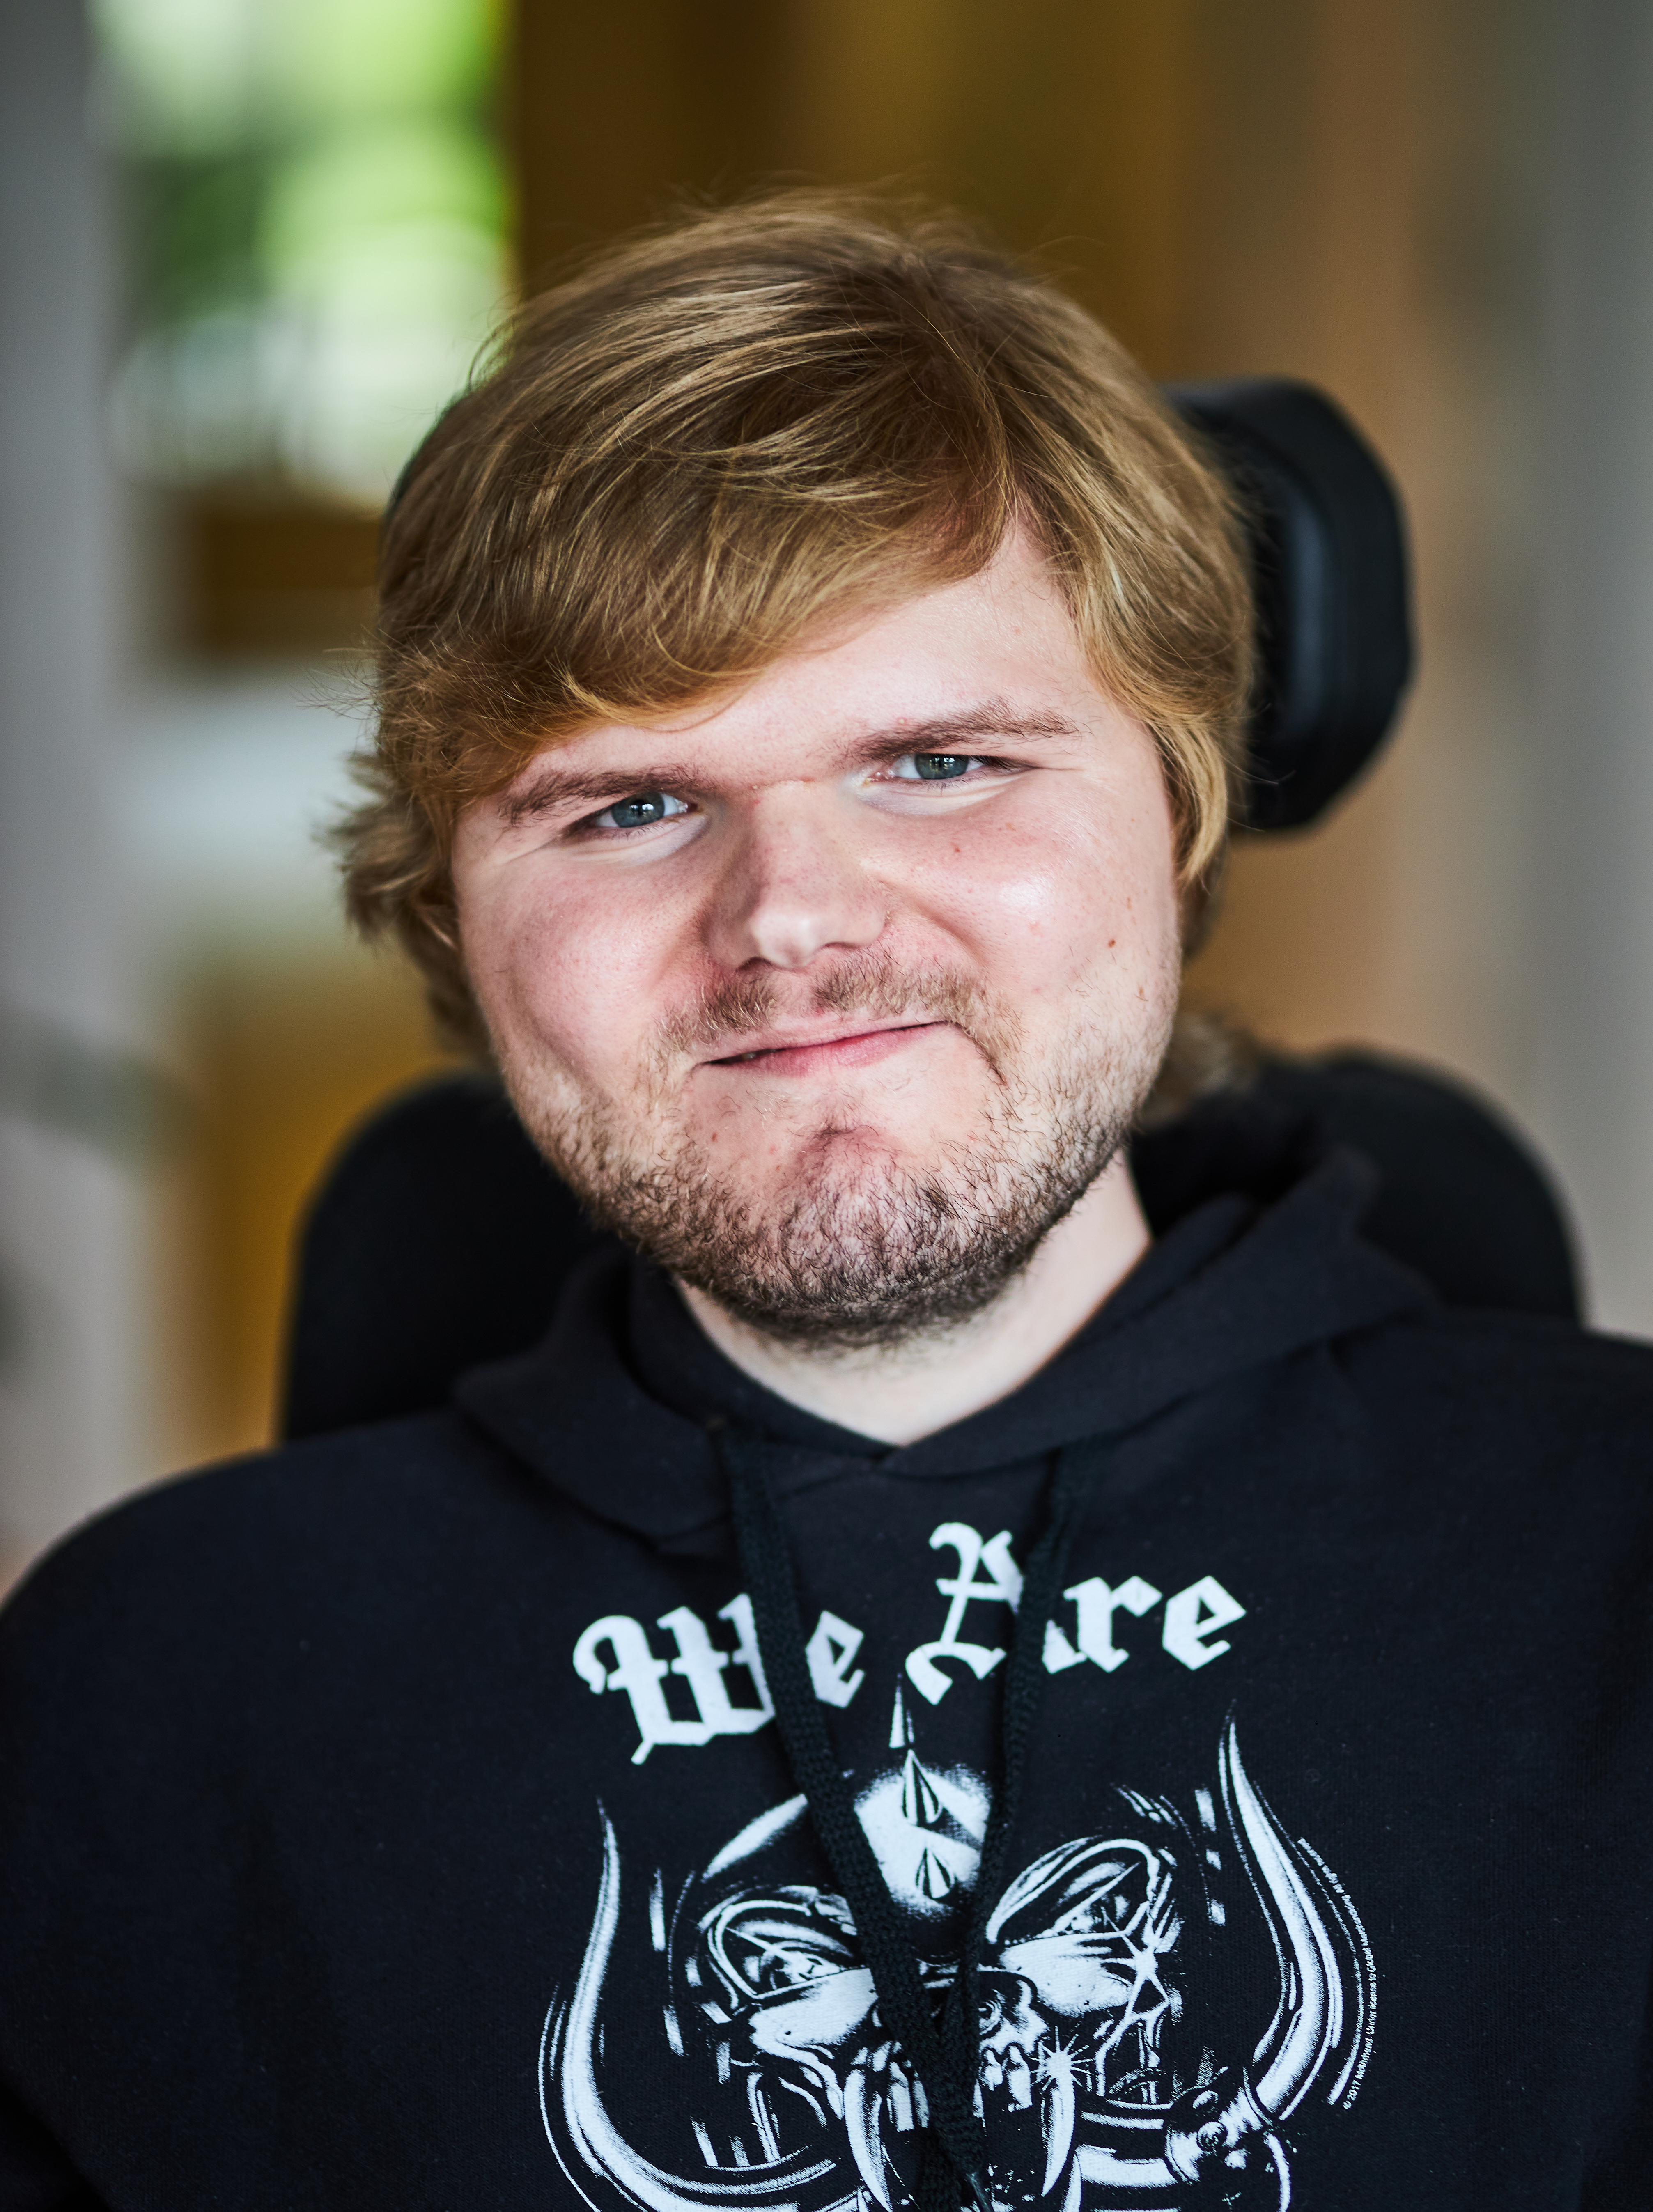
\includegraphics[width=0.45\textwidth]{Fotos/Marius.jpg}
\end{figure}
\noindent\small\textit{Grevenbroich, September 2024}

%\clearpage
%\tableofcontents % Hier wird das Inhaltsverzeichnis eingefügt
%\clearpage

\mainmatter

\clearpairofpagestyles % Setzt alle Kopf-/Fußzeilen zurück
\rehead{\leftmark}     % Gerade Seiten: Kapitelüberschrift rechts
\lehead{\thepage}      % Gerade Seiten: Seitenzahl links
\rohead{\thepage}      % Ungerade Seiten: Seitenzahl rechts
\lohead{\leftmark}     % Ungerade Seiten: Kapitelüberschrift links

\pagestyle{scrheadings}

\addchap{Die ersten Jahre}
\thispagestyle{scrheadings} % Wichtig, sonst erscheint die Kopfzeile nicht auf der ersten Seiet des Kapitels
\addcontentsline{toc}{chapter}{Die ersten Jahre}

\leavevmode
%\vspace*{0.5\baselineskip}
{\noindent\fontsize{18}{24}\selectfont\textcolor{myblue}{Ich, Wunschkind}\par}
{\noindent\fontsize{14}{20}\selectfont\scshape\textcolor{myblue}{Eigentlich lief alles bestens}\ldots\par}
\vspace*{0.5\baselineskip}
\normalsize

\noindent Was ist deine früheste Kindheitserinnerung? Und wie alt warst du da? Man sagt, dass die Grenze für früheste Erinnerungen zwischen drei und vier Jahren liegt. Um euch also über meine ersten Lebensjahre berichten zu können, musste ich meine Eltern, Elke und Peter, interviewen. Wir drei haben ein sehr gutes und inniges Verhältnis zueinander. Und meine Fragen über diese Phase meines Lebens haben sie gerne und ausführlich beantwortet. Apropos: falls ihr euch fragt – ich bin Marius, 29 Jahre alt.

Offenbar war ich ein lang ersehntes Wunschkind. Meine Eltern hatten sich jedenfalls riesig gefreut, als feststand, dass meine Mutter mit mir schwanger war. So wie sich alle Eltern freuen, die sich ein Kind wünschen. Die ersten drei Monate einer Schwangerschaft sind ja die kritischsten. Wie man nachlesen kann, übernimmt die Plazenta etwa ab der 12. Schwangerschaftswoche die vollständige Versorgung des Fötus. Danach sinkt das Risiko einer Fehlgeburt drastisch. Dementsprechend vorsichtig war meine Mutter während dieser Zeit und gab besonders gut auf uns beide acht. Wir kamen gut durch diese Phase und auch die übrigen 26 Wochen der Schwangerschaft.

Auf die Welt kam ich schließlich im Mai 1995 im Kreißsaal des Elisabeth-Kran\-ken\-hau\-ses in Grevenbroich. Auf den Tag genau, so wie es die Geburtsberechnung vorausgesagt hatte. Ich kam mit dem Kopf voran und mein jetziges, dunkelblondes Haar war bei der Geburt und auch einige Wochen danach noch schwarz. Getauft wurde ich auf den Namen Marius. Im Wettstreit der Vornamen hatten die Konkurrenten Oskar und Luis das Nachsehen. Zum Glück. Denn ist es nicht so, hat man erst einmal einen Vornamen, kann man sich einen anderen irgendwie nicht mehr vorstellen?

Apropos Namen: Den Namen Grevenbroich habt ihr vermutlich schon einmal gehört. Grevenbroich ist diese kleine Stadt, gelegen auf der linken Rheinseite im Dreieck Köln-Düsseldorf-Mönchengladbach, die bei Umweltschützern wegen der Braunkohleförderung im riesigen Tagebau Garzweiler zu zweifelhaftem Ruhm gekommen ist. 2030 soll damit Schluss sein. Grevenbroich wurde aber auch durch die von Hape Kerkeling verkörperte Kunstfigur Horst Schlämmer, seines Zeichens nuschelnder Chefredakteur des fiktiven Grevenbroicher Tagblattes, deutschlandweit bekannt.

\begin{figure}[ht]
    \centering
    \includegraphics[width=\textwidth]{Fotos/Grevenbroich_in_Google_Earth.png}
    \caption{Grevenbroich hat etwa 67.000 Einwohner und liegt im Braunkohlerevier westlich von Köln. Die ockerfarbenen Flecken auf der Karte sind Tagebaue, riesige, hunderte Meter tiefe Löcher, in denen gigantische Schaufelradbagger Braunkohle fördern.}
    \label{fig:grevenbroich}
\end{figure}

In diesem Städtchen also, genauer gesagt in seinem südlichsten Stadtteil Neurath, lebe ich seit meiner Geburt gemeinsam mit meinen Eltern, Kater Smokie sowie dem langhaarigen holländischen Hütehund Gonzalo. Ich war das erste Kind meiner Eltern und sollte auch das einzige bleiben. Nach Neurath kamen meine Eltern im November 1990, etwa fünf Jahre vor meiner Geburt. Beide sind gebürtige Grevenbroicher. Sie lebten bereits seit drei Jahren zusammen und hatten sich wegen einer aus ihrer Sicht unverschämten Mieterhöhung auf die Suche nach einem eigenen Haus gemacht. In Neurath wurden sie schließlich fündig.

Das Haus, in dem ich die ersten acht Jahre meines Lebens verbracht habe, ist eine zweieinhalbgeschossige Doppelhaushälfte aus den 50er Jahren. Keine Schönheit, aber einigermaßen gut in Schuss. Zum Zeitpunkt meiner Geburt gehörten auch die Bernhardiner-Dame Bianca und die beiden Kater Max und Felix mit zur Familie. Bianca litt leider an einem bösartigen Knochentumor am vorderen Lauf, der sich nicht operieren ließ. Mit vier Jahren haben meine Eltern sie auf Anraten des Tierarztes einschläfern lassen. Eine Erinnerung an sie habe ich nicht. Allerdings gibt es ein Foto, das sie neben meinem Kinderwagen sitzend zeigt. Mit den beiden Katern habe ich noch einige Jahre zusammen verbracht. Hunde und Katzen gehören von Anfang an zu meinem Leben. Sie haben mir immer viel Freude bereitet und mich oft zum Lachen gebracht. Ich bin fest davon überzeugt, dass Haustiere das Leben ihrer Besitzer positiv beeinflussen.

\setlength{\fboxsep}{0pt}    % Kein Abstand zwischen Rahmen und Bild
\setlength{\fboxrule}{0.2pt} % Rahmenstärke auf 0.2 pt setzen
\begin{figure}[ht]
    \centering
    \fcolorbox{rahmenlinie}{white}{\includegraphics[width=1\textwidth]{Fotos/Zeltgemeinschaft.jpg}}
    \caption{Der Schapendoes-Rüde Rudi hat mich viele Jahre begleitet. Aufgenommen wurde das Foto an einem Strand in der niederländischen Provinz Zeeland. Ein Leben ohne Haustiere ist für mich unvorstellbar.}
    \label{fig:zeltgemeinschaft}
\end{figure}

Zurück zum Haus. Wenn meine Eltern gewusst hätten, dass ihr Kind früher oder später auf einen Rollstuhl angewiesen wäre, hätten sie sich nicht für dieses Haus entschieden. Sie haben es aber weder gewusst noch haben sie es geahnt. Wie auch? Nichts deutete in den ersten zwei Jahren meines Lebens darauf hin. In Sachen Barrierefreiheit war das Haus eine Katastrophe. Mein Kinderzimmer, das mein Vater während der Schwangerschaft hergerichtet hatte und das von meinen Eltern liebevoll eingerichtet worden war, lag direkt unter dem Dach, zwei ziemlich steile Treppen vom Erdgeschoss entfernt. Ich kann mich noch daran erinnern, dass ich mich diese Treppen mühsam hinaufgeschleppt habe, beide Hände das Geländer fest umklammernd. Meine Schritte beim Treppensteigen waren dabei nicht alternierend. Das bedeutet, dass ich den ersten Fuß auf eine Stufe gesetzt habe und anschließend den zweiten Fuß auf dieselbe und nicht etwa auf die nächsthöhere Stufe. Ein typisches Anzeichen für eine Muskelschwäche.

Der Zugang zum Haus stellte ebenfalls eine Hürde dar, denn selbst das Erdgeschoss befand sich nicht auf Straßenniveau. Wie bei vielen Häusern, die in den 50er und 60er Jahren gebaut worden waren, musste man erst ein paar Stufen erklimmen, bevor man vor der Haustür stand. Und auch in den Garten kam man nur über eine Treppe. Von der reinen Quadratmeterzahl her bot das Haus locker Platz für bis zu vier Personen. Aber die Wohnfläche verteilte sich auf drei Etagen. Rollstuhl, Treppenlift, Aufzug? Undenkbar.

Die ersten zwei Jahre meines Lebens waren unspektakulär. Ich lernte nach und nach alle Familienmitglieder kennen, wurde auf Familienfeiern herumgereicht, aß und trank gut und wuchs zu einem Wonneproppen heran, der sich in nichts von anderen zweijährigen Wonneproppen unterschied.

\vspace{0.5\baselineskip}

\noindent Zumindest nicht auf den ersten Blick.

\section{Da stimmt was nicht}
Rückblickend betrachtet, so meine Mutter, gab es sehr wohl Anzeichen. Allerdings subtile, die man als Argloser nicht unbedingt zu deuten vermochte. Ich krabbelte beispielsweise nicht, so wie es viele (wenn auch nicht alle) Kleinkinder tun, bevor sie laufen lernen. Und ich war seit meinem ersten Lebensjahr heiser. In einer Situation fiel meiner Mutter auch auf, dass es mich Kraft kostete, wenn ich auf dem Bauch lag und den Kopf anheben wollte. Aber da ich schließlich mit 16 Monaten das Laufen erlernte, lösten sich diese ersten Bedenken, dass mit mir körperlich vielleicht etwas nicht stimmte, erstmal in Luft auf.

Meine Mutter hatte mich ein halbes Jahr nach meiner Geburt bereits in einem Kindergarten angemeldet, den ich mit dreieinhalb Jahren dann auch besuchte. Ein Jahr zuvor bin ich bereits regelmäßig in eine Spielgruppe gegangen (in der ich meinen ältesten Freund Marvin kennengelernt habe, zu dem ich heute noch Kontakt halte, auch wenn er zwischenzeitlich nach Berlin gezogen ist).

Gegen Ende meiner Zeit in dieser Spielgruppe fiel einer der beiden Pädagoginnen auf, dass ich offensichtlich Plattfüße und einen Watschelgang hatte. Beides sind Anzeichen für Duchenne Muskeldystrophie. Diese Art zu gehen, entsteht aufgrund der Schwäche der Hüft- und Gesäßmuskulatur. Um die Schwäche in der Hüfte auszugleichen und eine möglichst stabile Körperhaltung einzunehmen, machen Duchenne-Jungen ein Hohlkreuz und wölben den Bauch nach vorne. Wenn man in dieser Haltung barfuß geht, Plattfüße hat, weil das Fußgewölbe nicht richtig ausgebildet ist, und man den Fuß auch nicht abrollen kann, dann hat dieser Gang etwas von Watscheln. Duchenne Muskeldystrophie erkläre ich euch auf Seite 119 *** noch genauer.

\subsection{„Ach was! Das kommt noch!“ Denkste!}

Auch wenn man diese Fehlhaltung anfangs vielleicht noch mit einem „Ach was! Nicht alle Kinder sind gleich flink und beweglich. Das kommt schon noch!“ abtut, so schaut man nach einem solchen Fingerzeig vielleicht doch etwas genauer hin. Während man anfangs noch darüber hinwegsah, so waren die eigentümliche Körperhaltung mit vorgewölbtem Bauch und der tapsige Gang spätestens von da an unübersehbar geworden. Aber sie waren längst noch nicht beunruhigend. Wofür gibt es schließlich Physiotherapeut:innen? Man riet uns denn auch, eine solche aufzusuchen, um den Plattfuß und die vermeintlich daraus resultierende Fehlhaltung (wie meine Eltern fälschlicherweise glaubten) frühzeitig zu behandeln.
              
\subsection{Gowers-Manöver und die Schwierigkeit aufzustehen}

Alles gut? Leider nicht. Denn es wurde immer offensichtlicher, dass ich meinen Altersgenossen körperlich immer mehr hinterherhinkte. Vom Boden aufzustehen, fiel mir besonders schwer. Ich musste mich immer erst hinknien und dann mit dem Arm am Oberschenkel hochdrücken, um in den aufrechten Stand zu kommen. Diese Art sich aufzurichten, wird als Gowers-Manöver bezeichnet. Es ist typisch für Duchenne Muskeldystrophie.

\setlength{\fboxsep}{0pt}    % Kein Abstand zwischen Rahmen und Bild
\setlength{\fboxrule}{0.2pt} % Rahmenstärke auf 0.2 pt setzen
\begin{figure}[ht]
    \centering
    \fcolorbox{rahmenlinie}{white}{\includegraphics[width=1\textwidth]{Fotos/gowers-manöver.jpg}}
    \caption{Als Gowers-Manöver bezeichnet man die typische Art, wie sich Patienten mit einer Rumpfmuskelschwäche aus der Bauchlage in den Stand aufrichten. Zeichnung: Thomas Ebel}
    \label{fig:gowers-manöver}
\end{figure}

\subsection{Ich kann nicht so schnell}

Eine Situation hat sich bei meiner Mutter besonders eingeprägt. Wir hatten mit der Spielgruppe eine Waldwanderung unternommen und die Kinder trafen nach und nach am vereinbarten Ort ein, um von ihren Eltern in Empfang genommen zu werden. Die letzten, die dort viele Minuten nach den anderen ankamen, waren meine Spielgefährtin Janine und ich, gefolgt von einer erwachsenen Begleiterin. Ich konnte einfach nicht so schnell. Gehen kostete mich Kraft und ich stolperte auch immer häufiger, weil ich meine Füße beim Gehen nicht mehr ausreichend anheben konnte.

Als sich meine Eltern auf Anraten der Pädagogin dieser Spielgruppe dazu entschlossen hatten, mit mir einen Physiotherapeuten aufzusuchen, war es aus ihrer Sicht eigentlich nur eine Frage der Zeit, bis meine Beeinträchtigungen auskuriert wären und ich zu meinen Altersgenossen körperlich wieder aufschließen würde.

\subsection{Physiotherapie half auch nicht}

Nach einer Reihe von Physiotherapie-Sitzungen stellte sich der erhoffte Erfolg jedoch nicht ein. Die erste Praxis behandelte nach dem Ansatz von Bobath. Diese Methode wird bei Erwachsenen und Kindern mit neurologischen Erkrankungen angewendet, zum Beispiel bei Menschen, die nach einem Schlaganfall halbseitig gelähmt sind. Das Konzept beruht auf der Annahme, dass sich das Gehirn umorganisieren lässt, dass gesunde Hirnregionen Aufgaben neu lernen und übernehmen können, die zuvor von erkrankten Hirnregionen ausgeführt worden waren. Duchenne ist jedoch keine neurologische Erkrankung, von daher änderte die Behandlung natürlich auch nichts an meinem Zustand.

Man riet meinen Eltern, es mit einem anderen physiotherapeutischen Ansatz zu versuchen. Bei der Vojta-Therapie sollen Bewegungsstörungen durch eine Stimulation, nämlich das Auslösen von Reflexen, also auf einen bestimmten Reiz hin stets gleich ablaufende Reaktionen, die nicht bewusst gesteuert werden können, behoben werden. Für Vojta gilt das gleiche wie für Bobath: Duchenne ist eine muskuläre Erkrankung, die körperlichen Beeinträchtigungen sind Folge eines Absterbens von Muskelzellen – Reflextherapien beheben solche muskulären Defekte nicht.

Die dritte Physiotherapeutin (diese Praxis betreut mich übrigens bis heute) riet uns schließlich, mein Problem besser einmal medizinisch begutachten zu lassen. Der Kinderarzt, der mich von Geburt an behandelte und meine Eltern beraten hatte, war zwischenzeitlich in den Ruhestand gegangen. So vereinbarten sie einen Termin bei einem Kinderarzt, der seine Praxis in Grevenbroich gerade neu eröffnet hatte. Ihm erzählten sie also im Dezember 1998 meine Geschichte und dass keine der Physiotherapien auch nur eine leichte Besserung bewirkt hatte.

\subsection{Das Ende der unbeschwerten Jahre}

Der Arzt entnahm mir eine Blutprobe und ließ sie im Labor untersuchen. Wir hatten vor, das Weihnachtsfest und den Jahreswechsel gemeinsam mit meinen Großeltern im Erzgebirge zu verbringen. Meine Eltern erwähnten dies dem Arzt gegenüber wohl mehr oder weniger beiläufig. Denn obwohl das Ergebnis der Blutuntersuchung bereits vor unserer Abreise feststand, teilte man es meinen Eltern sozusagen aus Rücksicht auf ein paar unbeschwerte Feiertage erst nach unserer Rückkehr am 11. Januar 1999 mit.

Der Creatinkinase Wert (CK) in meinem Blut war deutlich erhöht. Das Enzym Creatinkinase ist für den Energiestoffwechsel der Muskelzellen wichtig. Sind die Zellen geschädigt, etwa durch einen Herzinfarkt, Sturz oder wie in meinem Fall durch das Fehlen des Proteins Dystrophin (daher auch der Name Muskeldystrophie), findet sich vermehrt Creatinkinase im Blut. Der Normalwert liegt bei einem Gesunden in meinem Alter bei weniger als 150 Einheiten pro Liter Plasma. Bei mir waren es 7.000. Die unbeschwerten Jahre waren damit vorbei.

Was die Diagnose Duchenne Muskeldystrophie bedeutete, war mir natürlich nicht klar. Aber von dem Moment der Diagnose an änderte sich mein Leben und das meiner Eltern schlagartig und dauerhaft. Ihnen wurde der Boden unter den Füßen weggezogen. Unser altes Leben, das noch wenige Wochen zuvor unbekümmert und glücklich war, rückte mit einem Schlag unwiederbringlich in weite Ferne und wurde zu etwas langsam Verblassendem, an das sie sehnsüchtig zurückdachten. Es sollten zwei Jahre vergehen, bis der Horror zumindest teilweise verarbeitet worden war und das Glück nach und nach in unsere Familie zurückkehrte.

\subsection{Was tun? Aktion Benni \& Co.}

Was tun Eltern, die soeben erfahren haben, dass ihr nicht einmal vier Jahre alter Sohn an einer fortschreitenden und tödlich verlaufenden Muskelkrankheit litt? Meine beschäftigten sich von dem Moment an intensiver mit dieser Krankheit. Beim Stöbern im Internet (Google war damals übrigens gerade mal ein Jahr alt) stießen sie auf die im Westerwald beheimatete Elterninitiative Aktion Benni \& Co. Diese war 1996, also ein Jahr nach meiner Geburt, von den Eltern des ebenfalls an Duchenne Muskeldystrophie erkrankten Benni gegründet worden.

Ziel der Initiative war es, Geld zu sammeln, um damit die Forschung in Bezug auf eine Heilung der Duchenne Muskeldystrophie zu intensivieren. Aktion Benni \& Co. ist mittlerweile in dem eingetragenen Verein Duchenne Deutschland e.~V. aufgegangen.

\begin{mdframed}[
    linewidth=0.3pt,         % Dünne Linie
    linecolor=rahmenlinie,   % Deine definierte Rahmenfarbe
    leftmargin=0, rightmargin=0,
    innertopmargin=12pt, innerbottommargin=12pt,
    innerleftmargin=12pt, innerrightmargin=12pt,
    backgroundcolor=white
]
\small\sffamily
\setlength{\parindent}{0pt} % Kein Erstzeileneinzug

\textbf{Duchenne Deutschland e.\,V. und Deutsche Duchenne Stiftung}

\vspace{0.5\baselineskip}

\textbf{Duchenne Deutschland e.~V.} ist eine Initiative von Eltern, deren Kinder Duchenne Muskeldystrophie (DMD) haben. Mit seiner Arbeit, die größtenteils von ehrenamtlichen Helfern geleistet wird, unterstützt der Selbsthilfeverein Betroffene und ihre Familien durch Beratung und Information in allen Lebensphasen.

\vspace{0.8\baselineskip}

Zweck des Vereins ist auch die Förderung von Wissenschaft und Forschung. Mit Spendengeldern unterstützt er – in Absprache mit einem wissenschaftlichen Beirat – die DMD-Forschung sowie Studien und fördert die Kommunikation und die Zusammenarbeit der weltweit mit DMD befassten Wissenschaftler. Der Verein informiert Patienten und ihre Familien über aktuelle und geplante Forschungsprojekte und richtet Veranstaltungen wie das jährliche Duchenne-Symposium oder regelmäßige Web-Konferenzen aus.

\vspace{0.8\baselineskip}

Die \textbf{Deutsche Duchenne Stiftung} (\url{https://www.duchenne-deutschland.de}) wurde 2010 als selbständige Stiftung gegründet, um die Arbeit für die Duchenne-Gemeinschaft dauerhaft zu sichern, die Forschung zur Entwicklung von Therapien zu forcieren und die Lebenssituation der Betroffenen zu verbessern. Aufklärung der Öffentlichkeit sowie die Umsetzung sozialer und psychologischer Projekte für DMD-Familien sind weitere Bestandteile der Stiftungsarbeit.

\vspace{0.8\baselineskip}
\textbf{Deutsche Duchenne Stiftung – Duchenne Deutschland e.~V.}

Huestraße 20, 44787 Bochum\\
Telefon: +49 234 925 696 70\\
Fax: +49 234 925 696 72\\
E-Mail: info@duchenne-deutschland.de\\
Webseite: \url{https://www.duchenne-deutschland.de}

\vspace{0.8\baselineskip}
\textbf{Spendenkonten}

Duchenne Deutschland e.~V.\\
Sparkasse Bochum\\
IBAN: DE67 4305 0001 0000 4277 24\\
BIC: WELADED1BOC\\
Deutsche Duchenne Stiftung\\
Volksbank Ruhr Mitte\\
IBAN: DE44 4226 0001 0603 1297 00

\end{mdframed}

\vspace{0.8\baselineskip}

\noindent Auch wenn Duchenne Muskeldystrophie die häufigste muskuläre Erbkrankheit im Kindesalter ist und statistisch etwa jeder 3.500ste Junge an ihr erkrankt, ist ihre Häufigkeit dennoch verschwindend gering im Vergleich zu Erkrankungen des Herz-Kreislauf-Systems, Krebs oder Diabetes. Alleine im Jahr 2020 gab es über eine halbe Million neudiagnostizierte Krebserkrankungen.

Für Pharmaunternehmen ist der Markt der Volkskrankheiten deutlich lukrativer als der eher übersichtliche Markt der neuromuskulären Erkrankungen wie Duchenne. Mit der kostspieligen Entwicklung von Medikamenten und Therapien lässt sich in diesem Segment schlicht kein Geld verdienen, und als Folge davon kommt auch die Forschung zu kurz. Und wenn an Duchenne Muskeldystrophie nicht geforscht wird, dann wird es weder mittelfristig noch langfristig Hoffnung auf Heilung geben.

Das möchten in Deutschland Vereine wie seinerzeit Aktion Benni \& Co., heute Duchenne Deutschland e.~V., oder in den USA Parent Project DMD ändern: sie machen die Öffentlichkeit auf die Krankheit aufmerksam und sammeln Spendengelder zur Unterstützung der Forschung mit Blick auf eine Heilung der Erkrankung.

Meine Eltern traten also dem Verein Aktion Benni \& Co. bei. Sie machten in und um Grevenbroich auf die Krankheit Duchenne Muskeldystrophie aufmerksam und sammelten fleißig Spendengelder. Damit begann eine Zeit mit vielen Benefizveranstaltungen, Fototerminen und Scheckübergaben. Wir tauchten in etlichen Zeitungsartikeln auf und machten mit unserer Geschichte das Thema Duchenne Muskeldystrophie einer größeren Öffentlichkeit bekannt.

Dies hatte dann auch den gewünschten Schneeballeffekt zur Folge: Denn nicht nur unsere Familien waren eifrig dabei, Spendengelder zu sammeln, auch Freunde und Bekannte legten sich mächtig ins Zeug, um unser Anliegen publik zu machen. Sie sprachen ihre Freunde, Bekannten und auch Firmen an und sorgten schließlich dafür, dass innerhalb von zwei Jahren mehr als 100.000 DM aus unserem Postleitzahlbezirk auf das Spendenkonto von Aktion Benni \& Co. eingezahlt wurden!

\setlength{\fboxsep}{0pt}    % Kein Abstand zwischen Rahmen und Bild
\setlength{\fboxrule}{0.2pt} % Rahmenstärke auf 0.2 pt setzen
\begin{figure}[ht]
    \centering
    \fcolorbox{rahmenlinie}{white}{\includegraphics[width=1\textwidth]{Fotos/Zeitungsausschnitte.jpg}}
    \caption{Unsere Geschichte wurde um die Jahrtausendwende in zahlreichen Zeitschriften veröffentlicht und machte das Thema Duchenne lokal und regional einer größeren Öffentlichkeit bekannt. Viele Menschen spendeten Geld. Innerhalb von etwa zwei Jahren gingen 100.000 DM aus unserem Postleitzahlbezirk auf dem Spendenkonto von Aktion Benni \& Co. ein.}
    \label{fig:zeitungsausschnitte}
\end{figure}

Meine Eltern erzählten mir, dass ihnen die vielen Aktivitäten rund um Aktion Benni \& Co. zwar nicht dabei halfen, die Realität um sie herum komplett auszublenden und den Horror ganz zu vergessen, man sah mir die Krankheit ja an, für deren Bekämpfung sie Spendengelder sammelten. Aber es lenkte sie zumindest ab. Sie hatten eine Aufgabe, auf die sie ihre Gedanken fokussieren konnten. Und mit jeder gespendeten (damals noch) DM, so hofften sie, würde auch die Heilung ihres Sohnes ein Stück näher rücken. Die beiden engagierten sich etwa zwei Jahre für Aktion Benni \& Co. und beschlossen dann, sich wieder mehr auf die Familie, auf uns drei zu konzentrieren. Dafür gab es einen guten Grund: Wir planten den Bau eines behindertengerechten Hauses.

\section{Wir bauen ein Haus}

Rückblickend war 2001 ein wirklich besonderes Jahr, weil in jenen 12 Monaten so viel passiert ist. Zum einen war im Spätsommer die Zeit des sorglosen Spielens, Bastelns und Singens im Kindergarten „Villa Kunterbunt“ vorbei. Ich war im Mai sechs geworden und kam in die Schule, so wie viele andere Sechsjährige auch. Ich kann mich nicht mehr daran erinnern, ob ich mich auf die Schule gefreut habe oder aber der Kindergartenzeit hinterhertrauerte. Wahrscheinlich tat ich beides. Von meiner Schulzeit werde ich später noch berichten. Zunächst möchte ich euch von dem bis dahin größten Projekt meiner Eltern erzählen, dem Bau eines behindertengerechten Hauses.

Ich kann mir vorstellen, dass es eine ganz besondere Herausforderung ist, ein Haus zu planen und zu bauen. Man bindet sich nicht nur für viele Jahre an eine Bank, sondern man entscheidet auch, wo man in Zukunft leben möchte und wo sich das Leben der Familie abspielen wird. Meine Eltern entschieden sich, in Neurath zu bauen.

Die Doppelhaushälfte in Neurath, die die beiden 1990 gekauft hatten und in der sie insgesamt 13 Jahre lang lebten, war acht Jahre lang mein Zuhause. Das Haus war Mitte der 50er Jahre gebaut worden und architektonisch nicht unbedingt ein Schmuckstück. Aber das können die wenigsten Häuser aus dieser Zeit von sich behaupten. Es verfügte über einen hübschen, kleinen Garten, in dem ein alter Kirschbaum stand, an dessen dickem Ast eine Schaukel hing, die mein Vater aus einem abgefahrenen Autoreifen und einem Seil gebaut hatte. Am Ende des Gartens befand sich ein ziemlich großes Gartenhaus, das sowohl auf unserem als auch auf dem Grundstück unserer Nachbarn stand, und das meine Eltern gemeinsam mit den Nachbarn schon vor meiner Geburt gebaut hatten. Unser Haus lag ziemlich zentral, etwas abseits der Dorfmitte Neuraths, nicht weit entfernt vom Kindergarten und direkt gegenüber der Grundschule.

\subsection{Unser erstes Zuhause, das Gegenteil von barrierefrei}

So sehr wir drei unser Zuhause auch liebten, hatte es doch einen gravierenden Nachteil: Es war das genaue Gegenteil eines behindertengerechten und barrierefreien Hauses. In der Zeit, als es gebaut wurde, war der Begriff „Barrierefreiheit“ noch nicht im Duden aufgeführt, und ob man mit dem Rollstuhl in ein öffentliches oder privates Gebäude kam, interessierte vor 70 Jahren niemanden. Zum Teil auch heute noch nicht.

Natürlich hatte ich als kleiner Junge überhaupt keine Ahnung, was Barrierefreiheit bedeutete und ebenso wenig wusste ich, dass die beengten Verhältnisse in unserem Haus für eine:n Rollstuhlfahrer:in ein echtes Problem darstellten. Ich war klein, hatte ganz andere Dinge im Kopf und konnte ja schließlich noch laufen. Allerdings ahnte ich damals schon, dass mit dem Haus irgendetwas nicht stimmt. Ich konnte zwar trotz der allmählich schwindenden Muskulatur in meinen Beinen noch im Erdgeschoss umherlaufen (und fiel dabei das eine oder andere Mal auch hin), ich schaffte es jedoch nicht, aus eigener Kraft in mein Kinderzimmer im zweiten Stock zu gelangen. Zwar kämpfte ich mich in ganz jungen Jahren noch alleine die Stufen hoch, später jedoch war es ganz selbstverständlich, dass meine Eltern mich die beiden steilen Treppen in mein Zimmer hochtrugen. Heruntersteigen konnte ich die Treppen anfangs noch alleine. Allerdings auch das nie, ohne dass meine Eltern danebenstanden, um auffangen zu können, falls ich stolperte. Damit musste man bei mir immer rechnen.

\subsection{Meine Angst vor Rollstühlen}

Mit der Diagnose Duchenne Muskeldystrophie stand unweigerlich fest, dass ich früher oder später einen Elektro-Rollstuhl brauchen würde, um mich eigenständig fortbewegen zu können. Ein Thema, das meine Eltern anfangs komplett ausgeblendet hatten. Mich im Rollstuhl sitzen zu sehen, war etwas, mit dem sie sich in den ersten beiden Jahren nach der Diagnose nicht befassen wollten oder konnten. Der Rollstuhl war nicht nur ein Hilfsmittel zur Fortbewegung und zum Erhalt der Selbstständigkeit. Er war auch ein Symbol. Ein Symbol dafür, dass mit dem Verlust meiner Gehfähigkeit für alle sichtbar das nächste Stadium der Krankheit begonnen hatte. Mit dem Rollstuhl würde eine neue Phase in meinem Leben anbrechen, die ich von da an im Sitzen und auf Rädern meistern musste, ob ich wollte oder nicht. Das zu akzeptieren, fiel anfangs nicht nur meinen Eltern schwer, sondern mir auch. Denn ich hatte Angst vor Rollstühlen.

Klingt komisch, aber war tatsächlich so. Es gibt eine Situation, die mir heute fast wie eine sich selbst erfüllende Prophezeiung vorkommt (ich bin allerdings nicht abergläubisch). Meine Eltern waren immer schon bekennende Camper. Eigentlich sind sie es immer noch, aber leider machen die Umstände das Zelten so gut wie unmöglich, der logistische Aufwand ist einfach riesig. Früher, als ich noch gehen konnte, aber auch noch, als ich schon im e-fix saß, haben wir viele unserer Urlaube und verlängerten Wochenenden an der holländischen Küste auf einem Campingplatz in der Nähe vor Domburg verbracht. Dazu auf Seite 67 *** mehr.

Es war vielleicht im Sommer 1999 oder 2000, als ich auf diesem Campingplatz zum ersten Mal einen Jungen in einem Elektro-Rollstuhl sah. Der Rollstuhl erschien mir riesig und er machte mir Angst. Anders als ich und alle anderen Menschen, die ich kannte, ging der Junge nicht auf zwei Beinen, sondern er fuhr mit diesem Ding umher, das zu allem Schrecken dieses seltsam summende Geräusch von sich gab. Ich konnte kaum hinschauen und ging dem Jungen falls möglich aus dem Weg. Dass ich keine zwei Jahre später selbst auf einen Rollstuhl angewiesen sein würde (zumindest zeitweise), ahnte ich natürlich nicht. Es würde zur Ironie des Schicksals passen, wäre der Junge so wie ich an Duchenne Muskeldystrophie erkrankt und ich sozusagen einen Blick meiner eigenen Zukunft erhascht hätte. So viel zur Angst vor Rollstühlen. Klar, die Angst war spätestens verschwunden, als ich selbst in einem saß.

\subsection{Treppen und Rollstuhl? Unmöglich.}

Doch zurück zum Haus. Auch wenn meine Eltern das Thema Rollstuhl emotional auf Distanz hielten, so war ihnen doch schon mit der Diagnose klar, dass das Haus ein Problem darstellte, mit dem man sich früher oder später befassen musste. Spätestens dann, wenn sich abzeichnete, dass ich einen Rollstuhl bräuchte.
Doch welche Optionen gab es? Die auf den ersten Blick naheliegendste war ein Umbau des Hauses. Doch das war nicht so einfach, um nicht zu sagen unmöglich. Das Erdgeschoss hatte eine Fläche von etwa 50 Quadratmetern und bot Platz für ein Wohnzimmer, ein Gäste-WC und die Küche. Es lag gut einen Meter über Straßenniveau und war nur über eine Außentreppe erreichbar. Diesen Niveauunterschied hätte man mit einer langen Rampe überwinden können. Doch mit welchem Ergebnis? Ich wäre mit dem Rolli zwar ins Haus gekommen, aber spätestens dort wäre mit der Barrierefreiheit Schluss gewesen.

Wie gesagt, es war alles ziemlich beengt und wichtige Räume wie Bad und Kinderzimmer lagen im ersten bzw. zweiten Obergeschoss. Wie sollte ich im Rollstuhl dorthin kommen? Dafür hätte man einen Außenaufzug benötigt. Auch den hatten meine Eltern in Erwägung gezogen. Allerdings gab es keine geeignete Wand, an die man den Aufzug von außen hätte montieren und wo man die Fassade hätte durchbrechen können, um ins Hausinnere zu gelangen. Selbst wenn, so wäre ein Aufzug bautechnisch nur bis ins erste Obergeschoss möglich gewesen. Bis unter das Dach, wo mein Kinderzimmer lag, hätte man ihn nicht bauen können. Es wurde meinen Eltern recht schnell klar, dass Aufwand und Nutzen eines solchen Vorhabens in keinem vernünftigen Verhältnis standen. Ein Außenaufzug hätte sehr aufwändige und teure Umbaumaßnahmen im Hausinneren erforderlich gemacht und wäre doch immer ein fauler Kompromiss geblieben, über den man sich später ärgern würde.

\subsection{Entscheidung Neubau}

Am Ende entschieden sie sich dazu, neu zu bauen. Und zwar in Neurath. Für meine Eltern war es damals wichtig, dass wir dortblieben. Eine Entscheidung, die sie heute zwar nicht unbedingt bereuen, die sie aber unter Umständen nicht mehr so treffen würden. Einer der wichtigsten Gründe, nicht aus Neurath wegzuziehen, war das soziale Umfeld, in dem ich groß geworden war. Ich besuchte den dortigen Kindergarten und lernte in den drei Jahren viele Kinder kennen, mit denen ich auch nachmittags oft spielte. Außerdem wechselte ich ja auf die Grundschule in Neurath, wo ich viele meiner Spielgefährt:innen aus der Kindergartenzeit wieder treffen würde.

Im Kreise all der Kinder, die mich und meine Krankheit schon aus der Kindergartenzeit kannten, wäre ich gut aufgehoben, so dachten meine Eltern damals, als diese wichtige Entscheidung anstand. Der Tatsache, dass sich die Wege nach der Grundschulzeit in der Regel trennen, hatten sie dabei weniger Beachtung geschenkt. Ehemalige Spielgefährt:innen oder Klassenkamerad:innen laufen mir in Neurath jedenfalls so gut wie nie über den Weg. Vielleicht wäre ein Umzug zum Beispiel nach Köln besser gewesen, weil in einer großen Stadt einfach mehr los ist und man dort fast alles mit öffentlichen Verkehrsmitteln erreichen kann. Für einen Umzug nach Köln hätten meine Eltern auch auf ihr soziales Netz, auf die Nähe zu ihren Familien und zu ihrem Freundeskreis verzichten müssen, bei denen wir uns geborgen fühlen und die uns in vielerlei Hinsicht unterstützt haben. Außerdem wäre jeder Besuch bei meinen Großeltern in Grevenbroich zu einem Tagesausflug geworden.

Neurath ist ein kleines Dorf, das von den meisten Grevenbroichern wegen seiner Lage in unmittelbarer Nähe der Braunkohlekraftwerke eher abschätzig betrachtet wird. Und von der Stadtverwaltung erhält es leider auch nicht die (finanzielle) Zuwendung, die es eigentlich bräuchte. Aber die Menschen, die hier leben, sind toll. Jedenfalls die, die ich im Laufe der Jahre kennengelernt habe.

Ich war ungefähr sieben Jahre alt und saß schon zeitweise im Rollstuhl, als ich darauf angesprochen wurde, ob ich nicht Lust hätte, Mitglied in der Artillerie Neurath zu werden. Die Artillerie ist ein Schützenzug, bei dem nicht nur Erwachsene mitmachten. Sie hatte auch eine Kinderabteilung, die Jung-Artillerie, in die einige meiner Schulkameraden eingetreten waren. Wir fuhren regelmäßig ins Kino, machten viele Ausflüge und traf uns oft zum Grillen. Während der Schützenfestumzüge saßen die Erwachsenen auf einer großen und die Kinder auf einer kleinen Kanone, die von Traktoren durchs Dorf gezogen wurden. Das war für mich natürlich praktisch, denn ich musste nicht wie die anderen Schützen zu Fuß marschieren.

\setlength{\fboxsep}{0pt}    % Kein Abstand zwischen Rahmen und Bild
\setlength{\fboxrule}{0.2pt} % Rahmenstärke auf 0.2 pt setzen
\begin{figure}[ht]
    \centering
    \fcolorbox{rahmenlinie}{white}{\includegraphics[width=1\textwidth]{Fotos/Schützenfest 2002.jpg}}
    \caption{Ich auf der Kanone der Artillerie Neurath sitzend. In späteren Jahren wurde ich sicherheitshalber mit einem Gurt an der Sitzbank befestigt. Im Hintergrund sieht man übrigens den Traktor, mit dem die Kanone der Erwachsenen gezogen wird.}
    \label{fig:schützenfest}
\end{figure}

Anfangs bin ich noch selbst auf die Kanone geklettert, später dann, als meine Kräfte mich mehr und mehr verließen, wurde ich von einem der Erwachsenen auf die Kanone gehoben. Die Umzüge haben viel Spaß gemacht und ich habe mich immer darauf gefreut! Leider war eine Fahrt auf der Kanone nach meiner Wirbelsäulen-Operation, von der ich euch auf Seite 133 berichten werde, nicht mehr möglich. Die Kanone war nicht gefedert und jede Unebenheit im Boden, hätte meine Wirbelsäule erschüttert und die an den Wirbelkörpern befestigten Stangen lösen können. Mitgefahren bin ich aber trotzdem, und zwar uniformiert in meinem Rollstuhl direkt neben der Kanone! Noch heute bin ich passives Mitglied in der Artillerie und werde von den Jungs jedes Jahr besucht. Zum Auftakt des Schützenfestes kommen sie mit der Kanone bei mir vorbei und wir böllern das Fest mit ein paar lauten Schüssen ein.

Wenn wir drei heute darüber reden und uns fragen, ob wir nicht besser fortgezogen wären, dann sind wir immer noch hin und hergerissen zwischen dem Leben, das wir heute führen, und dem Leben, das wir zum Beispiel in Köln hätten führen können. Ironischerweise bin ich nach der Grundschule auf die Anna-Freud-Schule in Köln gewechselt (http://www.anna-freud-schule.de/). Mein Schulweg wäre deutlich kürzer gewesen, hätte ich damals in Köln statt in Neurath gewohnt. So aber hat mich jeden Morgen ein Fahrdienst zuhause abgeholt, nach Köln-Müngersdorf gebracht und nachmittags dort wieder abgeholt. Trotzdem: Mir persönlich tut die Entscheidung jedenfalls nicht leid. Ich fühle mich auf dem Land wohl. Außerdem sind Köln und Düsseldorf ja nicht weit. Und wenn die S-Bahn-Linie 6 Grevenbroich-Köln kommt (hoffentlich bald und hoffentlich mit barrierefreiem Zugang zum Gleis und in den Zug), dann sind wir in gerade mal 30 Minuten in der Domstadt.

\subsection{Auf Grundstücksuche}

Kurz noch ein paar Worte zu dem Dorf, in dem ich lebe: Neurath liegt am südlichsten Rand des Rhein-Erft-Kreises, gut 10 km vom Zentrum des Städtchens Grevenbroich entfernt. Der Ort ist seit vielen Jahrzehnten vom Braunkohletagebau und den großen Braunkohlekraftwerken geprägt. Aus deren riesigen Kühltürmen kondensieren kilometerhohe Wasserdampf-Schwaden, die man noch aus 50 km Entfernung sehen kann. Die unmittelbare Nähe zu diesen Kraftwerken macht Neurath nicht gerade zu einem attraktiven Ortsteil. Das Gegenteil ist der Fall. Wenn man nicht aus dieser Ecke stammt und in unmittelbarer Nähe der gewaltigen Industriekomplexe groß geworden ist, dann stößt einen die Kraftwerkskulisse ab. In Neurath schießen deshalb auch keine neuen Baugebiete aus dem Boden wie in anderen Ortsteilen, und frei bebaubare Grundstücke in guter Lage sind äußerst rar. Wenn man dann auch noch plant, einen ebenerdigen Bungalow zu bauen, dann stellt der Mangel an Grundstücken mit geeigneter Größe ein echtes Problem dar. Vor genau diesem standen meine Eltern 2001.

In Neurath gab es schlicht kein Grundstück, auf das man einen Bungalow hätte bauen können. Zumindest keines, das erschlossen war. Aber wie der Zufall es will, öffnete sich genau zu diesem Zeitpunkt ein Türchen. Von einer Bekannten, die gehört hatte, dass wir bauen wollten, erfuhr meine Mutter von einer völlig verwilderten Brachfläche am Ortsrand von Neurath. Sie lag abgelegen und versteckt hinter den letzten Häusern des Dorfes und war schätzungsweise 5.000 Quadratmeter groß. Wenn überhaupt, dann kannten vielleicht ein paar Hundebesitzer, die mit ihren Vierbeinern in dieser Gegend spazieren gingen, diese Parzelle, die komplett verwuchert war und sich in Besitz des RWE befand. Meine Eltern, die zu diesem Zeitpunkt schon über 10 Jahre in Neurath lebten, kannten sie jedenfalls nicht.

\subsection{Der Zufall klopft an}

Die Bekannte erzählte meiner Mutter, ihr sei zu Ohren gekommen, dass RWE plante, diese Fläche in ein paar Jahren in Bauland umwandeln zu lassen. Noch am gleichen Tag stand mein Vater auf der Parzelle und machte sich vor Ort ein Bild. Das Grundstück war ein Traum. Es lag geschützt hinter einem ehemaligen Bahndamm direkt an einem Waldstück (Neurath hat mehr grüne Ecken als man denkt) und hatte etwas Dornröschenhaftes an sich, weil es von Sträuchern und Büschen restlos zugewachsen war. Man brauchte nicht viel Phantasie, um sich vorzustellen, dass dies ein optimales Gelände für eine kleine Siedlung mit vielleicht 10 Häusern wäre.

Das war im Frühjahr 2001, und die Aussicht auf ein Baugrundstück war eine Gelegenheit, die man beim Schopf packen musste. Wenn RWE ohnehin vorhatte, in ein paar Jahren und in Abstimmung mit der Stadt Grevenbroich aus der Brachfläche Bauland zu machen, dann ließe sich diese Entscheidung unter Umständen beschleunigen? Das konnte man nur herausfinden, indem man RWE und die Stadt Grevenbroich anschrieb und die Situation schilderte. Eigentlich mussten nur zwei Fragen beantwortet werden: Würde RWE die Parzelle eventuell vor dem bislang geplanten Zeitpunkt verkaufen und falls ja, würde die Stadt Grevenbroich dann einer Erschließung des Geländes zustimmen und sie gegebenenfalls sogar beschleunigen? Vielleicht wäre es ja sogar möglich, dass wir bereits im kommenden Jahr mit dem Neubau beginnen könnten. Es war möglich.

Die Nachricht erreichte uns im Sommer 2001, nur wenige Monate nach der ersten Kontaktaufnahme. Wir verbrachten gerade unseren Urlaub in Südspanien. Es war der letzte Urlaub in „Freiheit“, ab August ging ich ja zur Schule. Der Urlaub bleibt meinen Eltern in zweifacher Hinsicht in Erinnerung. Ich wäre nämlich beinahe im Außenpool unseres Hotels in Andalusien ertrunken. Ich sprang in einem unbeobachteten Moment ins Wasser, ohne zu wissen, dass ich nicht schwimmen konnte. Meine Mutter döste vor sich hin, hörte jedoch zum Glück das Platschen, als ich im Wasser landete. Nach einigen Sekunden fiel ihr dann auf, dass es still war und sie mich nicht mehr reden hörte. Da lief sie in Panik zum Beckenrand und sah mich dort senkrecht treibend, den Kopf unter Wasser. Sie packte mich an einem Arm und zog mich heraus. Adrenalin pur. Wie ihr seht, habe ich es überlebt. Glück gehabt!

An einem Tag während dieses Urlaubs rief uns meine Tante an. Sie hatte während unserer Abwesenheit unseren Briefkasten geleert und dabei einen Brief vom RWE entdeckt. Wir baten sie, uns den Inhalt vorzulesen. RWE teilte uns darin freudig mit, dass man die Parzelle schnellstmöglich veräußern würde und bereits Kontakt zur Stadt Grevenbroich aufgenommen habe. Vom Bauamt hatten wir vorab schon die Zusage erhalten, dass man sich für eine zügige Erschließung der Fläche einsetzen werde, sobald RWE diese verkaufen würde. Der Bebauungsplan müsse hierfür allerdings zunächst angepasst und dann veröffentlicht werden, was noch ein paar Monate dauern könne und tatsächlich auch ein halbes Jahr dauerte.

Noch am Tag des Anrufs begannen die Planungen. Meine Mutter hatte in der Nacht vor lauter Aufregung kein Auge zugemacht und damit begonnen, einen ersten Grundriss zu zeichnen. Von diesem ist, wie zu erwarten, am Ende kaum etwas übriggeblieben. Allerdings wurde das Wohnkonzept so umgesetzt, wie meine Eltern es sich vorgestellt hatten. Mittelpunkt unseres häuslichen Lebens ist eine 40 Quadratmeter große Küche. Hier spielt sich fast alles ab.

\setlength{\fboxsep}{0pt}    % Kein Abstand zwischen Rahmen und Bild
\setlength{\fboxrule}{0.2pt} % Rahmenstärke auf 0.2 pt setzen
\begin{figure}[ht]
    \centering
    \fcolorbox{rahmenlinie}{white}{\includegraphics[width=1\textwidth]{Fotos/Baugrube.jpg}}
    \caption{Mein Vater und ich in der Baugrube.}
    \label{fig:baugrube}
\end{figure}

Als wir zurück in Deutschland waren, begannen die konkreten Planungen. Zuallererst brauchten wir einen Architekten, der das Wohnkonzept, das meinen Eltern vorschwebte, umsetzen konnte. Zum Glück mussten wir diesen nicht lange suchen. Volker war ein Klassenkamerad meines Vaters und hatte sich als Architekt einen Namen gemacht. Aufträge für 08/15 Entwürfe (Haustür, Flur, links Gäste-WC und Treppenaufgang Obergeschoß, rechts Küche, hinten Wohnzimmer und Garten) lehnte er ab, wenn er konnte. Das Projekt "Barrierefreier Bungalow" reizte ihn hingegen umso mehr, außerdem war er ein alter Freund der Familie und wollte uns helfen. Beim Preis kam er uns auch entgegen.

\subsection{Der Bagger kommt}

Die Bauarbeiten begannen im Juni 2002. Ich war natürlich live dabei, als der Bagger seine Schaufel zum ersten Mal in den Boden stieß und begann, den Keller unseres Hauses auszuheben. Meine Eltern und ich sind RWE und der Stadt Grevenbroich noch heute dankbar dafür, dass sie das Gelände unkompliziert und schnell in Bauland umgewandelt, die Erschließung und Parzellierung vorangetrieben und die Grundstücke schließlich uns und acht weiteren Interessenten zum Kauf angeboten haben. Wir würden heute nicht in Neurath leben und unser Leben wäre ganz anders verlaufen.

Der Bau zog sich über ein Jahr hin, und größere Probleme gab es zum Glück keine. Im August 2003 zogen wir ein. Bis auf die Treppe in den Keller hat das Haus keine Stufen. Der Zugang von der Straße ist ebenerdig ebenso wie alle Ausgänge in den Garten. Beim Ausheben der Baugrube hatte man diese Anforderung bereits berücksichtigt und das Loch entsprechend tief gegraben. Jeder Raum ist für mich erreichbar. Selbst die Räume im Keller. Das Haus verfügt nämlich über einen Aufzug. Mein Zimmer und das sich daran anschließende Bad liegen im Erdgeschoss und sind beide genauso geräumig wie die Küche. Neben einem Heizungs- und Vorratsraum befinden sich im Keller ein Büro, das ich mir mit meinem Vater teile, das Gym meines Vaters sowie mein Zockerzimmer mit den diversen Spielekonsolen, die sich im Laufe der Jahre angesammelt haben. Hierhin ziehen wir uns zurück, wenn meine Freunde Marco und Marvin zu Gast sind, und machen dabei auch schon mal die Nacht durch (einmal sogar zwei Nächte hintereinander). Unser Haus steht für Freunde immer offen. Sie sind hier jederzeit willkommen.

\addchap{Schule, Ausbildung und Job}
\thispagestyle{scrheadings} % Wichtig, sonst erscheint die Kopfzeile nicht auf der ersten Seiet des Kapitels
\addcontentsline{toc}{chapter}{Schule, Ausbildung und Job}

\leavevmode
%\vspace*{0.5\baselineskip}
%{\noindent\fontsize{18}{24}\selectfont\textcolor{myblue}{Ich, Wunschkind}\par}
%{\noindent\fontsize{14}{20}\selectfont\scshape\textcolor{myblue}{Eigentlich lief alles bestens}\ldots\par}
%\vspace*{0.5\baselineskip}
\normalsize

 \section{Meine Grundschulzeit}

Meine Kindergartenzeit endete mit einer schönen Abschiedsfeier irgendwann im Juni 2001. Kinder, Eltern und Betreuer:innen trafen sich noch ein letztes Mal, tauschten bei Kaffee und Kuchen Erinnerungen und Anekdoten aus und wünschten sich alles Gute für die Zukunft. Manch eine:r verdrückte dabei die eine oder andere Träne, und dann war einfach Schluss. Die Kindergartenzeit war Vergangenheit, und ich würde die Räume, in denen ich fast drei Jahre mit anderen gespielt hatte, nie wieder betreten. Allerdings dauerte die Trennung von meinen ehemaligen Spielkamerad:innen nicht besonders lange. Viele von ihnen sah ich bereits wenige Wochen später wieder, in der Klasse 1 der Grundschule Neurath.

\subsection{Kindergarten oder Schule}

Es stand nicht von Anfang an fest, dass ich im September 2001 die Grundschule besuchen würde. Ich war zwar im Mai sechs geworden und hatte damit das offizielle Einschulungsalter erreicht, meine Eltern hatten es jedoch nicht unbedingt eilig, mich aus dem Kindergarten zu nehmen. Offenbar war ich für mein Alter noch etwas zu verspielt, daher dachten sie darüber nach, mich ein Jahr länger in der behüteten Umgebung des Kindergartens zu lassen.

Schließlich ließen wir doch meine Schulfähigkeit feststellen. Meine Eltern organisierten zu diesem Zweck einen Termin an der Universität Düsseldorf. Dort sollte von einem Spezialisten mithilfe eines kognitiven Tests geklärt werden, ob meine Entwicklung altersgerecht war und, falls dies der Fall wäre, einem Schulbesuch nichts im Wege stand. Bei einer kognitiven Beurteilung werden gewöhnlich Aspekte wie die Sprachentwicklung, Hör- und Sehfähigkeit, Konzentration und Wahrnehmung sowie die allgemeine altersgerechte Entwicklung berücksichtigt. Es gibt jedoch keine standardisierten Kriterien, denn jedes Kind ist einzigartig und eine dezente Schwäche in dem einen oder anderen Punkt heißt noch nicht, dass ein Kind nicht eingeschult werden kann. Mir wurde jedenfalls die Schulreife attestiert und so betrat ich an einem Montag Anfang September 2001, zusammen mit 20 weiteren Schüler:innen den Klassenraum der Klasse 1 der Grundschule Neurath.

Rückblickend bin ich froh, dass es genauso kam und ich nicht noch ein weiteres Jahr den Kindergarten besucht habe. Hierfür gibt es mehrere Gründe. Zum einen war die Leiterin des Kindergartens, zugleich Betreuerin meiner Gruppe, an einen anderen Kindergarten gewechselt. Zu ihr hatte ich ein besonders inniges Verhältnis, und ohne sie wäre es nicht mehr das gleiche gewesen. Außerdem waren viele der Spielkamerad:innen meiner Gruppe ja nicht mehr da, von ihnen hatte ich mich auf der Abschlussfeier im Juni bereits verabschiedet. Es erleichterte mir den Schulstart schon sehr, dass ich mit vielen der Kinder, mit denen ich wenige Wochen zuvor noch im Kindergarten gespielt hatte, am Ende dann doch gemeinsam die erste Klasse besuchte. Ich fühlte mich nicht so allein in dieser neuen Umgebung, sondern hatte vertraute Gesichter um mich. Ich denke, dieses Gefühl kennt jeder.

\subsection{Was wäre, wenn…}

Aber der eigentliche Grund, weshalb ich heute heilfroh darüber bin, meine Kindergartenzeit nicht in die Länge gezogen zu haben, ist ein anderer: Es wäre alles ganz anders gekommen! Jeder weiß ja aus eigener Erfahrung, dass wichtige Entscheidungen, die man in der Vergangenheit getroffen hat, den weiteren Lauf des Lebens oft maßgeblich beeinflussen. Also in meinem Fall kann ich das nur bestätigen. Meine schulische und berufliche Entwicklung wäre sehr wahrscheinlich eine komplett andere gewesen. Rückblickend betrachtet hat sich irgendwie alles wie von Zauberhand ineinandergefügt, beginnend mit meinem ersten Tag in der Grundschule, über die Zeit an der weiterführenden Schule, meine Ausbildung zum 3D-Produktdesigner bis hin zum meinem jetzigen Job. Ich bin mir ziemlich sicher, dass ich jetzt nicht hier sitzen und diese Zeilen schreiben würde, hätte sich mein Schulstart um ein Jahr verzögert. Alle Gelegenheiten, bei denen man die Weichen des Lebens stellen kann, bieten sich einem nur einmal. Mein "anderes" Leben wäre nicht zwangsläufig schlechter gewesen, aber definitiv anders.

Mit sechs Jahren war ich übrigens noch nicht auf einen Rollstuhl angewiesen. Ich habe ja schon erwähnt, dass das Haus, in dem wir seinerzeit wohnten, gleich gegenüber der Grundschule lag. Ich musste nur die Hauptstraße mit dem Zebrastreifen überqueren und befand mich nach weiteren 20 Metern schon auf dem Schulhof. Das war praktisch. Ich hatte mehr Zeit zum Rumtrödeln, was ich zum Ärger meiner Mutter das eine oder andere Mal auf die Spitze trieb. Einmal hatte ich den Bogen überspannt. Trotz mehrfacher Ermahnung ließ ich mir wieder mal Zeit. Bis ich dann die Pausenglocke hörte und mir schlagartig klar wurde, dass ich es nicht mehr rechtzeitig in den Klassenraum schaffen würde. Rennen konnte ich ja damals schon nicht. Als ich den Klassenraum betrat, war der Unterricht schon im Gange, und ich musste mir irgendeine Entschuldigung einfallen lassen. Ob sie glaubhaft war, daran kann ich mich nicht erinnern, wahrscheinlich war sie es nicht. Ich kam jedenfalls nie mehr zu spät.

\setlength{\fboxsep}{0pt}    % Kein Abstand zwischen Rahmen und Bild
\setlength{\fboxrule}{0.2pt} % Rahmenstärke auf 0.2 pt setzen
\begin{figure}[ht]
    \centering
    \fcolorbox{rahmenlinie}{white}{\includegraphics[width=1\textwidth]{Fotos/Schule (2).jpg}}
    \caption{Im ersten Schuljahr konnte ich noch gehen. Hier seht ihr mich rechts unten mit einigen meiner damaligen Klassenkamerad:innen beim Schmücken des Dorf-Weihnachtsbaumes.}
    \label{fig:schule2}
\end{figure}

\subsection{Die Schule zieht um}

Ich habe keine echte Erinnerung mehr an das erste Schuljahr. Ich weiß nur, dass es eigentlich gar nicht so schlimm war. Im zweiten Schuljahr stand uns allerdings eine große Änderung bevor. Das Gebäude, in dem die Grundschule Neurath untergebracht war, hatte man bereits 1913 errichtet. Nicht nur die Bausubstanz war schlecht, auch die Elektrik und die sanitären Anlagen waren in die Jahre gekommen und nicht mehr zeitgemäß. Eine Sanierung des Gebäudes hatte sich wegen des miserablen Zustandes nicht mehr gelohnt, weshalb man beschlossen hatte, in das Gebäude der ehemaligen Hauptschule Neurath umzuziehen, die wiederum in das Nachbardorf umgezogen war.

Für die Schulleitung war die Aussicht, in ein moderneres und größeres Gebäude umziehen zu können, natürlich ein Glücksfall. Den meisten Schüler:innen und deren Eltern wird es wahrscheinlich egal gewesen sein. Für mich wurde der nun 500 Meter lange Schulweg allerdings zum Problem, denn die Kraft in meinen Muskeln ließ nach. Zu Fuß schaffte ich diese Strecke nicht mehr. Es wurde Zeit für meinen ersten Rollstuhl. Dabei handelte es sich um einen manuellen Rollstuhl, der mit einem als e-fix bezeichneten elektrischen Zusatzantrieb versehen war (die Motoren saßen auf den Naben der Räder) und der per Joystick gesteuert werden konnte. Mit diesem Rollstuhl legte ich nun die Strecke von unserem Haus zur Schule zurück, fast immer begleitet von meinen Klassenkamerad:innen, die mich morgens zuhause abholten.

\subsection{Die neue Grundschule – Barrierefrei mit Einschränkung}

Mit dem Neubau unseres Hauses hatten wir zu diesem Zeitpunkt bereits begonnen, und das Problem "Barrierefreiheit" würde sich in unserem künftigen Zuhause nicht mehr stellen. Für die neue Schule, die in den 1960er Jahren gebaut worden war, galt dies jedoch nicht. Die Klassenräume befanden sich sowohl im Erdgeschoss als auch im ersten Obergeschoss, das nur über eine Treppe erreichbar war. Unsere Klasse war aus diesem Grund auch im Erdgeschoss untergebracht. Allerdings wurde das Fach Religion für zwei Klassen übergreifend unterrichtet, und weil sich deswegen die Anzahl der Schüler:innen verdoppelt hatte, musste ein größerer Raum her. Einen solchen gab es nur im ersten Stock. Also musste meine Mutter vor dem Unterricht zur Schule kommen, mich hochtragen, auf einem Stuhl "parken", dann den Rollstuhl hochschleppen, mich umsetzen und 45 Minuten später das gleiche in umgekehrter Reihenfolge erneut tun.

Wenn ich an meine Grundschulzeit zurückdenke, dann kommt es mir so vor, als sei meine Mutter fast täglich vor Ort gewesen, weil es irgendwie immer etwas zu erledigen gab. Mal war sie da, um mich für den Religionsunterricht im ersten Stock die Treppe hoch- und danach wieder runter zu tragen, oder auch um andere Hilfestellungen zu leisten. Mal kam sie vorbei, um mir Sachen zu bringen, die ich zuhause vergessen hatte, mal, um mich zum Sportunterricht zu bringen und umzuziehen oder mit den Lehrer:innen Dinge zu besprechen, die aufgrund meiner Krankheit etwas mehr Vorlauf in der Planung benötigten, beispielsweise Klassenausflüge.

\subsection{Auf Klassenfahrt}

Im dritten Schuljahr ging die Klassenfahrt in den Brückenkopf-Park in Jülich, eine Festungsanlage aus napoleonischer Zeit, etwa eine halbe Stunde Autofahrt von Grevenbroich entfernt. Dummerweise war der Bus, der unsere Klasse dorthin brachte und später wieder abholte, kein sogenannter Niederflurbus. Wie der Name vermuten lässt, handelt es sich bei Niederflurbussen um Fahrzeuge, die an den Eingängen keine Stufen zwischen der Straße und dem Boden der Fahrgastkabine haben, in die man also mit dem Rollstuhl rein- und rausfahren kann. Heutzutage ist dieser Typ von Bus Standard im öffentlichen Nahverkehr. Bei dem Bus, der für die Klassenfahrt eingesetzt wurde, gab es jedoch Treppen zum ein- und aussteigen und der Gang zwischen den Sitzreihen war so eng war, dass dort kein Rollstuhl zwischen passte. Also blieb meiner Mutter nichts anderes übrig, als mich mit unserem VW Bus in den Park zu fahren, wenn ich nicht zuhause bleiben sollte.

Im vierten und letzten Grundschuljahr ging die alljährliche Klassenfahrt dann mit dem Bus in die Eifel, in eine Jugendherberge, also mit Übernachtung. Damit war ich dann aus mehreren Gründen raus. Den Transport hätte meine Mutter noch übernehmen können, auch wenn Hellenthal mit einer Entfernung von 100 km nicht gerade ein Katzensprung ist.

Doch das eigentliche Problem war das Gebäude an sich. So schön und gepflegt das historische Fachwerkgebäude auch war, so wenig behindertengerecht war es leider auch. Der Eingang der Jugendherberge lag gut 2 Meter über Straßenniveau und war nur über eine Treppe erreichbar. Natürlich gab es auch keine Aufzüge. Offensichtlich verfügt sie heute über eine barrierefreie Etage für Rollstuhlfahrer:innen sowie behindertenfreundliche Zimmer (und hoffentlich auch WCs und Bäder).

\setlength{\fboxsep}{0pt}    % Kein Abstand zwischen Rahmen und Bild
\setlength{\fboxrule}{0.2pt} % Rahmenstärke auf 0.2 pt setzen
\begin{figure}[ht]
    \centering
    \fcolorbox{rahmenlinie}{white}{\includegraphics[width=1\textwidth]{Fotos/Schule (1).jpg}}
    \caption{Ab etwa dem zweiten Schuljahr benötigte ich dann einen Rollstuhl. Hier seht ihr mich in einem e-fix sitzend während einer Klassenfahrt im Wildfreigehege Hellenthal in der Eifel.}
    \label{fig:schule1}
\end{figure}

Wie man das Problem der Außentreppe für Rollstuhlfahrer:innen gelöst hat, konnte ich auf der Webseite nicht herausfinden. Selbst wenn die baulichen Bedingungen damals optimal gewesen wären, hätte auf jeden Fall eine Begleitung mitfahren müssen, um bei allem zu helfen, zu dem ich aufgrund meiner Muskelschwäche körperlich nicht mehr in der Lage war. Also ist meine Mutter am zweiten Tag mit mir nach Hellenthal gefahren, wo ich mit meinen Klassenkamerad:innen das Wildfreigehege besucht habe. Abends ging es dann für uns beide wieder nach Hause, während die anderen zurück zur Jugendherberge wanderten und einen weiteren Tag in Hellenthal blieben.

\subsection{Bundesjugendspiele}

Dass ich aufgrund meiner Erkrankung als Schüler keine Sportskanone war und auch niemals eine werden würde, das war klar. Ich hätte mich deshalb auch ohne weiteres vor den jährlich stattfindenden Bundesjugendspielen drücken können. Aber solange ich noch laufen konnte, wollte ich mich von der Krankheit auch nicht unterkriegen lassen. Also habe ich an dem Schülerwettbewerb teilgenommen, allerdings außerhalb der Wertung, denn an Punkte war bei meinen Leistungen beim Laufen, Weitsprung und Ballwurf nicht zu denken. Aber das war mir egal. Ich wollte auch eine Urkunde haben, so wie die anderen!

Die drei Disziplinen waren echte Herausforderungen. Mir fehlte die Kraft zum Laufen, wie sollte ich da springen? (Ich kann mich übrigens nicht daran erinnern, überhaupt jemals gesprungen zu sein.) Mit der Kraft, die ich in meinen Armen hatte, war ich gerade noch so in der Lage, den Ball ein paar wenige Meter weit zu schleudern. Von einem Wurf konnte man da nicht sprechen. Richtig schwer fiel mir jedoch das Laufen. Immerhin musste ich 50 Meter zurücklegen. Die Zeit, die ich dafür brauchte, spielte keine Rolle, viel wichtiger war, die gesamte Distanz durchzuhalten und nicht nach 20 Metern erschöpft aufzugeben. Zum Glück hatte ich Unterstützung: Meine Mutter lief neben der Bahn mit und feuerte mich an, so dass ich tatsächlich die Ziellinie erreichte. Natürlich war ich stolz, als ich die Urkunde entgegennehmen durfte. Es hat zwar nicht für eine Sieger- geschweige denn Ehrenurkunde, sondern nur für eine Teilnahmeurkunde gereicht, aber die habe ich mir hart erarbeitet.

\setlength{\fboxsep}{0pt}    % Kein Abstand zwischen Rahmen und Bild
\setlength{\fboxrule}{0.2pt} % Rahmenstärke auf 0.2 pt setzen
\begin{figure}[H]
    \raggedright
    \fcolorbox{rahmenlinie}{white}{\includegraphics[width=0.5\textwidth]{Fotos/Bundesjugendspiele.jpg}}
    \caption{Auch wenn es bei den Bundesjugendspielen nur für eine Teilnahmeurkunde gereicht hat, so war ich damals trotzdem stolz, diese entgegenzunehmen. Ich habe mich genauso abgerackert wie meine Mitschüler:innen. Ich hätte mich vor dem Schülerwettbewerb auch drücken können, aber kneifen gilt nicht.}
    \label{fig:bundesjugendspiele}
\end{figure}

\section{Die Anna-Freud-Schule in Köln}

Im Verlauf des vierten Schuljahrs bahnte sich ein Drama an, über das ich heute lächeln kann, das mir und meinen Eltern damals jedoch die Laune wochenlang verdorben hat. Es ging um das Thema "Empfehlung für die weiterführende Schule". Wie ich euch in einem separaten Kapitel auf Seite 130 noch erzählen werde, sind meine Eltern und ich nach der Diagnose Duchenne Muskeldystrophie regelmäßig zu Kontrolluntersuchungen in die Kinderklinik des Universitätsklinikums Düsseldorf gefahren. Meine behandelnde Ärztin dort war Dr. Jutta Gärtner. Sie ist 2002 an das Universitätsklinikum Göttingen gewechselt, wo sie mittlerweile eine Professur bekleidet. Bevor sie Düsseldorf verließ, diskutierten wir mit ihr die Frage, wo und von wem ich mich in Zukunft am besten behandeln lassen sollte. Sie empfahl uns Prof. Dr. Thomas Voit, damals Leiter der Klinik für Allgemeine Pädiatrie mit Schwerpunkt Neuropädiatrie an der Universitätsklinik Essen. Ein ausgewiesener Fachmann für neuromuskuläre Erkrankungen, der später an das Louis-Pasteur-Institut in Paris gewechselt ist und dort an Duchenne Muskeldystrophie geforscht hat.

\subsection{Der Tipp vom Professor}

Meine Gespräche mit ihm drehten sich natürlich in erster Linie um meinen Zustand. Er wollte wissen, wie es mir aktuell geht und ob sich Dinge seit dem letzten Besuch verschlechtert hatten. Aber ihn interessierte auch, welche Hobbys ich habe, wie es in der Schule läuft und auf welche weiterführende Schule ich denn im Anschluss an die Grundschule wechseln möchte. Für seine Empfehlung bezüglich der weiterführenden Schule bin ich ihm bis heute dankbar. Er empfahl mir, die Anna-Freud-Schule in Köln zu besuchen, eine Förderschule für körperliche und motorische Entwicklung des Landschaftsverbands Rheinland (LVR). Das Besondere an dieser Schule: Sie unterrichtet als einzige Förderschule für Körperbehinderte in NRW in der Sekundarstufe I (Fachoberschulreife) und in der Sekundarstufe II (Abitur).

\begin{mdframed}[
    linewidth=0.3pt,         % Dünne Linie
    linecolor=rahmenlinie,   % Deine definierte Rahmenfarbe
    leftmargin=0, rightmargin=0,
    innertopmargin=12pt, innerbottommargin=12pt,
    innerleftmargin=12pt, innerrightmargin=12pt,
    backgroundcolor=white
]
\small\sffamily
\setlength{\parindent}{0pt} % Kein Erstzeileneinzug

\textbf{Anna-Freud-Schule - Eine prozessorientierte, inklusive Schule}

\vspace{0.5\baselineskip}

Die LVR-Anna-Freud-Schule ist eine Förderschule des Landschaftsverbandes Rheinland in Köln (LVR) für Kinder und Jugendliche mit körperlichen Behinderungen sowie psychischen und psychosomatischen Erkrankungen.

\vspace{0.5\baselineskip}

Als einzige weiterführende Förderschule für Körperbehinderte in NRW unterrichtet sie in der Sekundarstufe I vorwiegend nach Realschulrichtlinien und in den Jahrgangsstufen EF, Q1 und Q2 (ehem. 11-13) nach den Richtlinien der gymnasialen Oberstufe mit der Möglichkeit, auch das Abitur zu machen. Die Schülerinnen und Schüler werden ganzheitlich gefördert. Pädagogen, Therapeuten und Pflegepersonal arbeiten eng zusammen und ermöglichen den Schülerinnen und Schülern eine umfassende und individuelle Förderung. Die Schule verfügt über eine eigene Turnhalle und ein eigenes Schwimmbad. Zurzeit besuchen rund 286 Schülerinnen und Schüler die LVR-Anna-Freud-Schule.

\vspace{0.5\baselineskip}

Für Schülerinnen und Schüler, die wegen ihrer Behinderung oder einer zu weiten Anfahrt nicht mit Bus und Bahn fahren können, hat der LVR einen Schülerspezialverkehr eingerichtet.

{\footnotesize Quelle: Anna-Freud-Schule (\url{http://www.anna-freud-schule.de/})}

\end{mdframed}

\vspace{0.8\baselineskip}

Natürlich hatten meine Eltern und ich uns bereits vor dem Gespräch mit dem Arzt viele Gedanken über die weiterführende Schule gemacht. Von einer solchen Entscheidung hängt ja später einmal viel ab, auch wenn man sich dessen nicht unbedingt bewusst ist. Doch während gesunde Kinder auf Basis des letzten Versetzungszeugnisses der Grundschule sowie der Empfehlung der Lehrkraft mehr oder weniger die freie Wahl zwischen Hauptschule, Realschule, Gesamtschule oder Gymnasium haben, sieht die Situation für körperbehinderte Kinder düster aus. Vor allem, wenn es sich wie in meinem Fall um eine schwere Behinderung handelt und man auf einen Rollstuhl und auf die Hilfe Dritter angewiesen ist.

In Grevenbroich kam nur die Käthe-Kollwitz-Gesamtschule in Betracht. Wir hatten bereits ein Gespräch mit dem Schulleiter dieser recht beliebten Schule geführt, und aus seiner Sicht sprach nichts dagegen. Auch wenn klar war, dass die räumlichen Bedingungen nicht optimal waren, so hätte ich diese Schule jedenfalls besuchen können. Nach dem Gespräch mit Prof. Dr. Voit war das Thema jedoch mehr oder weniger vom Tisch. Die Anna-Freud-Schule war immerhin eine weiterführende Schule speziell für Menschen wie mich. Außerdem war ihre Entfernung von meinem Wohnort mit 35 km noch im Rahmen, und für Schüler:innen, die wegen ihrer Behinderung nicht mit Bus und Bahn fahren konnten, wurde vom LVR auch der Transport geregelt. Ich wurde jeden Morgen um 6:40 von einem Fahrdienst abgeholt. Auf der Fahrt zur Schule sind wir weitere Orte angefahren, um andere Kinder mitzunehmen, manche von ihnen saßen so wie ich im Rollstuhl. Nach Schulschluss gegen 15:30 Uhr wurden wir dann wieder nach Hause gefahren. Die Fahrt dauerte gut eine Stunde.

\subsection{Nicht jeder kann die Anna-Freud-Schule besuchen}

Ein Wechsel auf die Anna-Freud-Schule war jedoch an mehrere Bedingungen geknüpft. Zum einen musste man einer Verordnung des Landes Nordrhein-Westfalen entsprechend den sonderpädagogischen Unterstützungsbedarf im Bereich körperliche und motorische Entwicklung gemäß der Ausbildungsordnung für Sonderpädagogische Förderung nachweisen. Das heißt, die körperliche oder motorische Behinderung musste beim Schulamt belegt werden. Zum anderen musste das Lehrerkollegium der Grundschule am Ende des vierten Schuljahres eine Empfehlung für die Realschule aussprechen. Zu guter Letzt musste man an der Anna-Freud-Schule auch noch einen Aufnahmetest erfolgreich bestehen. Dabei handelte es sich um den Hamburg-Wechsler-Intelligenztest für Kinder III, auch bekannt als HAWIK-III Test, mit dem die kognitiven Fähigkeiten von Kindern und Jugendlichen erfasst werden.

\begin{mdframed}[
    linewidth=0.3pt,         % Dünne Linie
    linecolor=rahmenlinie,   % Deine definierte Rahmenfarbe
    leftmargin=0, rightmargin=0,
    innertopmargin=12pt, innerbottommargin=12pt,
    innerleftmargin=12pt, innerrightmargin=12pt,
    backgroundcolor=white
]
\small\sffamily
\setlength{\parindent}{0pt} % Kein Erstzeileneinzug

\textbf{HAWIK-III}

\vspace{0.5\baselineskip}

Der Hamburg-Wechsler-Intelligenztest (HAWIK) ist ein Intelligenztest für Kinder und Jugendliche im Alter von 6 bis 16 Jahren. Er wurde von der Universität Hamburg entwickelt und basiert auf dem Wechsler Intelligence Scale for Children (WISC), einem weit verbreiteten Intelligenztest für Kinder. Der HAWIK untersucht verschiedene Aspekte der Intelligenz, wie zum Beispiel die Verarbeitungsgeschwindigkeit, die Gedächtnisleistung und die logischen Fähigkeiten. Der Test besteht aus verschiedenen Aufgaben und Übungen, die die Kinder lösen müssen, um ihre Intelligenz zu messen. Er wird oft von Psychologen und Pädagogen verwendet, um Kinder mit Lern- oder Verhaltensproblemen zu diagnostizieren und zu behandeln.

\end{mdframed}

\vspace{0.8\baselineskip}

Der sonderpädagogische Unterstützungsbedarf ließ sich in meinem Fall natürlich leicht nachweisen. Bei der Realschulempfehlung hatte meine damalige Klassenlehrerin jedoch Bedenken. Für meine Eltern und mich war das sowohl überraschend als auch in der Begründung vollkommen unverständlich.

\subsection{Nur mit Realschulempfehlung}

Obwohl mein Abschlusszeugnis mich für jeden Typ von weiterführender Schule qualifiziert hatte, traute meine Klassenlehrerin mir nicht zu - warum auch immer - dass ich die Realschule schaffen würde. Für diese Frau gehörte ich einfach nicht in die Kategorie Realschule. Meine Mutter kostete es einiges an Überredungskraft, um ihr klarzumachen, dass die Anna-Freud-Schule die beste Schule für mich sei. Würde ich die Aufnahmeprüfung dort nicht bestehen, hätte sich das Thema sowieso erledigt. Sie dürfe mir diese einmalige Chance jedoch nicht leichtfertig verwehren. Am Ende wurde die Realschulempfehlung ausgesprochen und ich bin stolz, dass ich es allen, die nicht an mich geglaubt haben, gezeigt habe!

\section{Allein in Köln}

Also besuchte ich ab dem 21. August 2006 die Anna-Freud-Schule in Köln, was mir anfangs in zweifacher Hinsicht schwerfiel. Zum einen war es das erste Mal, dass ich tagsüber längere Zeit von meinen Eltern getrennt war. Immerhin waren es fast 10 Stunden, und die Distanz zwischen Köln und Grevenbroich war so groß, dass meine Mutter nicht einfach mal so vorbeikommen konnte, wie sie es in der Grundschule öfter getan hatte, um Dinge mit den Lehrern zu regeln oder mir etwas vorbeizubringen, das ich zuhause vergessen hatte. Ich war in dieser Zeit auf mich alleine gestellt und musste mich alleine in einem fremden Umfeld zurechtfinden.
Das ist natürlich nichts wirklich Außergewöhnliches. Da muss jedes Kind durch, das von der Grundschule auf eine weiterführende Schule wechselt. Aber die räumliche Distanz machte es doch etwas schwieriger. Außerdem war ich Fremden gegenüber eher verschlossen, was es nicht einfach machte, wenn man von einem Tag auf den anderen nur noch von Fremden umgeben war. Viele meiner Mitschüler:innen saßen so wie ich im Rollstuhl.

\subsection{Keine Sonderbehandlung für Behinderte}

An der Anna-Freud-Schule geht es zu wie an anderen weiterführenden Schulen auch. Die Tatsache, dass sie eine Förderschule für Kinder mit körperlichen Behinderungen oder psychischen Erkrankungen ist, bedeutet nicht, dass man dort in Watte gepackt wird. Auch auf der Anna-Freud-Schule gab es Schüler:innen, die man mochte und mit denen man sich angefreundet hat, welche, mit denen man klarkam, und andere, denen man am liebsten aus dem Weg ging, weil sie immer einen dummen Spruch auf den Lippen hatten, wenn man ihnen begegnete.

\section{Das Konzept der Förderschule}

Trotzdem ist die Anna-Freud-Schule etwas Besonderes und ich bin entsetzt über die aktuelle politische Diskussion, ob man das Konzept der Förderschulen aufgeben soll und ob behinderte Kinder und Jugendliche stattdessen im Sinne von „echter“ Inklusion Regelschulen besuchen sollen. Einen solchen Vorschlag kann nur jemand machen, der nicht behindert ist und keine Ahnung davon hat, wie es ist, dauerhaft auf die Hilfe anderer angewiesen zu sein. Jemand, der nicht versteht, dass den Unterricht begleitende Therapien wie Ergotherapie, Logotherapie und Physiotherapie nur an speziell dafür ausgestatteten Schulen mit entsprechend ausgebildeten Fachkräften möglich sind. Viele Behinderte mit erhöhtem Förderbedarf würden an einer Regelschule untergehen, weil man ihnen aus Mangel an Mitteln, Ausstattung, Lehrkräften und Zeit keine individuelle Unterstützung zukommen lassen kann.

\subsection{Von „Zivis“ und „FSJ-lern“}

Begleitende Therapien, individuelle Förderung sowie Hilfe bei alltäglichen Dingen wie dem Toilettengang machen Schulen wie die Anna-Freud-Schule aus. Dort gab es zu meiner Zeit den „Zivi-Raum“, in dem sich 10 Zivildienstleistende und FSJ-ler - junge Menschen, die ein freiwilliges soziales Jahr (FSJ) absolvierten - aufhielten, um bei Bedarf Hilfe zu leisten. Ich fuhr mit dem Rollstuhl dorthin, um zu fragen, ob jemand Zeit hatte, mir bei einer Sache zu helfen, die ich aufgrund meiner Behinderung alleine nicht bewerkstelligen konnte. Wenn ich mal zur Toilette musste, dann hoffte ich inständig, in dem Raum jemanden anzutreffen. Manchmal war der Raum jedoch leer und ich hatte ein echtes Problem.

\section{Das Komplettprogramm: Physio-, Logo- und Ergotherapie}

Ich erhielt an der Anna-Freud-Schule jeweils zweimal wöchentlich Physiotherapie, Logopädie und Ergotherapie nach Bobath. Das Bobath-Konzept ist ein interdisziplinärer Ansatz. Das bedeutet, dass verschiedene medizinische Berufsgruppen wie Physiotherapeut:innen, Pflegekräfte, Ärzt:innen und Ergotherapeut:innen zusammenarbeiten. Die Therapie-Sitzungen dauerten jeweils 45 Minuten und fanden während des normalen Unterrichts statt. Die Zeit musste ich nachholen und mich selbst darum kümmern, was im Unterricht besprochen worden war. Manchmal fanden die Therapien auch während der Hausaufgaben-Stunden am Nachmittag statt. Dann verpasste ich zwar den Unterricht nicht, musste die Hausaufgaben jedoch nach meiner Rückkehr zuhause um 16:30 erledigen. Das war zeitweise echt anstrengend. An solchen Abenden war ich wirklich platt.

Die Physiotherapie zielte darauf ab, meine Eigenaktivität zu erhalten oder zu fördern. Ich stand regelmäßig in einem sogenannten Stehtrainer. Dabei handelt es sich um ein medizinisches Gerät, das in der Rehabilitation verwendet wird, um Patient:innen dabei zu helfen, das Stehen und Gehen wieder zu erlernen. Sie können meist elektrisch betrieben werden und haben unter­schiedliche Einstellmöglichkeiten, damit sie an die Bedürfnisse und Fähigkeiten der Patient:innen angepasst werden können. Natürlich konnte ich durch ein Stehtrainer nicht die Fähigkeit zu gehen wiedererlangen. Für den Kreislauf von Menschen, die tagsüber ausschließlich im Rollstuhl sitzen, ist es jedoch förderlich, ab und zu aufgerichtet zu werden, auch wenn dies wegen der eingeschränkten Beweglichkeit meiner Gelenke aufgrund der zunehmenden Kontrakturen meiner Muskulatur teilweise sehr schmerzhaft war.

Bei der Logopädie ging es darum durch Mund- und Zungen-Übungen die Mundmuskulatur zu trainieren. Dieser Bereich wird von Patienten mit Muskelerkrankungen manchmal vernachlässigt und sorgt dafür, dass die Aussprache wegen fehlender Spannung schlechter wird. In der Ergotherapie habe ich gebastelt, um meine Feinmotorik zu trainieren, aber mich auch mit alternativen Schreibtechniken wie Spracherkennungs- und Diktiersoftware beschäftigt. Zu meinen Therapien mehr auf Seite 141 ***.

\section{Ausbildung und Job}

Nicht jeder hat mit dem Tag seines Schulabschlusses auch eine genaue Vorstellung davon, wie es beruflich weitergehen soll. Mache ich eine Ausbildung, entscheide ich mich für ein duales Studium oder schlage ich eine akademische Laufbahn ein und besuche eine Hochschule? In meinem Fall kamen natürlich wegen der körperlichen Einschränkungen bestimmte Ausbildungen nicht in Frage, Tischler hätte ich z. B. nicht werden können. Dafür boten sich andere Ausbildungen jedoch geradezu an. Insbesondere die, bei denen der PC eine zentrale Rolle spielte. Mit dem PC hatte ich mich schon seit vielen Jahren beschäftigt. Das hat auch damit zu tun, dass mein Vater in der IT-Sparte eines großen Finanzunternehmens arbeitete und vorher als Autor Bücher zu vielen Themen rund um den PC geschrieben hatte. Ich bin sozusagen mit dem PC großgeworden und habe auch schon relativ früh einen besessen.

\subsection{Nur nicht entmutigen lassen}

Ich weiß von anderen Jungen mit Duchenne Muskeldystrophie, die sich gefragt haben, warum sie überhaupt zu Schule gehen sollen. Mit unserer Erkrankung würden wir doch ohnehin weder einen Ausbildungsplatz bekommen noch jemals einen Job haben und Geld verdienen, so ihr Argument. Auch wenn ich diesen Gedankengang grundsätzlich verstehen kann, so ließ ich mich doch nie von ihm entmutigen.

Anfangs nutzte ich den PC zum Spielen, wobei mich besonders Aufbauspiele interessierten, bei denen man etwas erschaffen konnte, sei es eine Stadt (Anno) oder wie im Falle von Roller Coaster eine Achterbahn in einem virtuellen Freizeitpark. Mit dem PC konnte ich Dinge kreieren, die ich mit meinen Händen nicht herstellen konnte.

\subsection{Der Zufall klopft erneut an}

Wie der Zufall es will, hatte sich mein Vater seinerzeit hobbymäßig mit einer Software beschäftigt, mit der sich Dinge in 3D modellieren ließen. Die Software heißt Blender und sie sollte mein Leben maßgeblich beeinflussen, was ich damals im achten Schuljahr, als ich mich zum ersten Mal mit dem Programm beschäftigte, noch nicht wissen konnte.

Das Thema Design fesselte mich immer mehr und ich hatte vor, später Mediengestalter zu werden. Nach der Schule suchte ich also erst einmal eine Ausbildungsstelle, verschickte eine Reihe von Bewerbungen und wurde auch zu Bewerbungsgesprächen eingeladen. Leider verliefen diese jedoch nicht so, wie ich mir das gewünscht hatte. Als etwas ungerecht empfand ich, dass ich in einem Fall einen Test absolvieren musste, bei dem ich mit der Hand Dinge entwerfen sollte, was einfach nicht ging. Ich kam jedenfalls nicht in nächste Runde.

\subsection{Nichts für mich. Das Berufsbildungswerk in Volmarstein}

Kurze Zeit später hatte ich ein Beratungsgespräch beim Arbeitsamt. Der zuständige Mitarbeiter war sehr kompetent. Er unterstützte mich in meinem Wunsch, eine Ausbildung zu machen und riet mir dazu, es einmal in Volmarstein zu versuchen. Volmarstein ist ein Berufsbildungswerk mit einem integrierten Internat, etwa 100 km von meinem Wohnort entfernt. Dort wurde eine Ausbildung zum Mediengestalter angeboten, was vom Berufsbild in die richtige Richtung ging. Also nahmen mein Eltern Kontakt mit der Einrichtung auf und vereinbarten eine Art Probezeit von vier Wochen.

Als der Tag gekommen war, reiste ich mit Sack und Pack an. Aber bereits nach wenigen Stunden, meine Eltern waren noch nicht zurückgefahren, stand für mich fest, dass ich dort nicht bleiben würde. Es gefiel mir überhaupt nicht und noch am Tag meiner Anreise reiste ich wieder ab. Man lernt in einem Internat zwar, selbstständig zu werden, aber gleichzeitig fühlte ich mich dort abhängiger als je zuvor. Vor allem, weil ich von allen Auszubildenden dort am meisten Hilfe gebraucht hätte. Ich hatte einfach kein gutes Gefühl bei der Sache.

Deshalb nahm ich mir vor, mich zunächst selbst um eine Ausbildungsstelle zu kümmern. Sollte ich nach einem Jahr immer noch mit leeren Händen dastehen, würde ich Volmarstein noch einmal eine Chance geben und die Ausbildung zum Mediengestalter dort antreten. Aber so weit kam es zum Glück nicht.

\subsection{Auf der Suche nach einem Ausbildungsplatz}

Die Suche nach einem Ausbildungsplatz dauerte fast ein Jahr. Es war ein Jahr ohne Struktur, ohne wirkliche Perspektive. Das ging mir furchtbar auf die Nerven. Ich war in dieser Zeit nicht besonders gut drauf, blieb lange im Bett und hatte zu nichts Lust. Doch bei einem Besuch der Messe REHACARE in Düsseldorf entdeckten meine Eltern und ich an einem Stand zufällig das E-Learning-Angebot des Berufsbildungswerks Neckargemünd. Man bot dort sogenannte E-Learning-Ausbildungen an, also Ausbildungen, die man von zuhause aus in virtuellen Klassenräumen machen konnte. Es gab zwar nur eine begrenzte Anzahl von Ausbildungsberufen, die sich dafür anboten, unter ihnen war jedoch auch der Beruf des Technischen Produktdesigners. Das war genau das, wonach ich suchte!

\subsection{Meine Ausbildung zum Technischen Produktdesigner 3D}

Im September 2013 begann ich endlich meine Ausbildung. Sie dauerte dreieinhalb Jahre. Ähnlich einer Videokonferenz wurde dabei virtuell gelehrt. Der Lehrer gab dabei seinen Bildschirm frei, der quasi die Tafel darstellte. In unserem Ausbildungsjahrgang waren wir nur zu dritt, da konnte man sich nicht verstecken. Natürlich gab es auch einen Stundenplan, Theorie und Praxis gingen Hand in Hand. Uns wurden Laptops und die Software zur Verfügung gestellt, allerdings gab es keine Ausbildungsvergütung. Zum Glück bekam ich von meinen Eltern Taschengeld, so dass ich mir das eine oder andere leisten konnte.

Anfang 2017 gab ich meine Abschlussarbeit ab. Die Aufgabe bestand darin, einen sogenannten Roboter-Parallelgreifer zum Versetzen von Paketen zu konstruieren. War nicht ganz so einfach, macht man schließlich nicht alle Tage. Es musste nicht nur ein 3D-Modell entworfen werden, das schön anzusehen war, es musste auch nachgewiesen werden, dass es funktioniert.

Es gab mehrere Möglichkeiten, einen solchen Robotergreifer auszuführen, z. B. mechanisch oder hydraulisch. Ich habe mich für die mechanische Ausführung entschieden, da wir Hydraulik in der Ausbildung nicht besprochen hatten. Es mussten Berechnungen zwecks Materialwahl und -stärke durchgeführt und alles fein säuberlich dokumentiert und eingereicht werden. Zu guter Letzt wurde ich in einer mündlichen Prüfung zu dem Projekt befragt. Auf jeden Fall habe ich die Prüfung erfolgreich bestanden und seit Februar 2017 bin ich Technischer 3D-Produktdesigner mit IHK-Abschluss. Wer einmal einen Blick auf meine Abschlussarbeit werfen möchte, kann dies unter \url{https://at.tumblr.com/topperdillon/robotergreiferpdf/hup54b91bple} tun.

Ich kann eine Ausbildung via E-Learning jedem, der an einer schweren Körperbehinderung wie Muskeldystrophie leidet, nur empfehlen. Natürlich ist es verlockend auszuziehen, um wirklich selbstständig und unabhängig von den Eltern zu sein. Ich wollte mich jedoch zunächst um einen Job kümmern und eventuell erst danach auszuziehen, um wirklich auf eigenen Füßen zu stehen, ohne dass meine Eltern am Ende doch für alles für bezahlen müssen.

\setlength{\fboxsep}{0pt}    % Kein Abstand zwischen Rahmen und Bild
\setlength{\fboxrule}{0.2pt} % Rahmenstärke auf 0.2 pt setzen
\begin{figure}[H]
    \raggedright
    \fcolorbox{rahmenlinie}{white}{\includegraphics[width=\textwidth]{Fotos/Blender (1).jpg}}
    \caption{Hier ein Gebäude, das ich für das Baustellenschild eines Neubaus modelliert habe.}
    \label{fig:baustellenschild}
\end{figure}

\setlength{\fboxsep}{0pt}    % Kein Abstand zwischen Rahmen und Bild
\setlength{\fboxrule}{0.2pt} % Rahmenstärke auf 0.2 pt setzen
\begin{figure}[H]
    \raggedright
    \fcolorbox{rahmenlinie}{white}{\includegraphics[width=\textwidth]{Fotos/Blender (2).jpg}}
    \caption{Und hier der Umbau eines Pfarrzentrums aus der Vogelperspektive.}
    \label{fig:pfarrzentrum}
\end{figure}

\subsection{Ausbildung abgeschlossen! Und jetzt?}

Ich hatte die Ausbildung zum Technischen Produktdesigner zwar mit Erfolg absolviert. Einen Job hatte ich aber trotzdem noch nicht. Es verging noch ein Jahr, bis es soweit war. Nach der Ausbildung musste ich zunächst wieder beim Arbeitsamt vorstellig werden und mich dort arbeitssuchend melden. Der Mitarbeiter, mit dem ich das Gespräch hatte (es war leider nicht derselbe, der mich vier Jahre zuvor bei der Suche nach einer Ausbildungsstelle unterstützt hatte), kam gleich zur Sache. Ich müsse womöglich in eine Werkstatt für Menschen mit Behinderung! Mir fiel die Kinnlade herunter und ich war wirklich verunsichert. Das erste, das diesem Herrn für meine berufliche Zukunft einfiel, war die Werkstatt für Behinderte? Dafür habe ich mich also dreieinhalb Jahre zum Technischen Produktdesigner ausbilden lassen? Selbst jetzt, sieben Jahre später, muss ich darüber noch den Kopf schütteln.

So traurig mich dieses Klischee auch machte (und immer noch macht), so sehr spornte es mich an, diesen Mitarbeiter und alle, die so denken wie er, vom Gegenteil zu überzeugen. Jetzt erst recht! Ich ergriff selbst die Initiative. Ich schrieb dutzende von Bewerbungen, vor allem an Architekten. Ich hatte mich in meiner Freizeit intensiv mit dem Thema Architekturvisualisierung in 3D beschäftigt und zahlreiche Projekte realisiert, die ich den Bewerbungen als Arbeitsproben beilegte. Leider ohne großen Erfolg. Entweder bestand kein Bedarf oder es scheiterte, wie in einem Fall, am Thema Toilettengang.

\subsection{Alleine pinkeln müsste man können…}

Ein Konstruktionsunternehmen in Mönchengladbach hatte auf eine Anfrage des Arbeitsamtes reagiert und sich tatsächlich bereit erklärt, mich einzustellen. Bis nach Mönchengladbach sind es von Grevenbroich aus nur knapp 30 km, maximal eine halbe Stunde Fahrt also. Das war schon mal sehr gut. Die Firma nutzte dann auch noch die Software, an der ich ausgebildet worden war. Das war wiederum äußerst hilfreich. Ich hätte sofort produktiv mitarbeiten können, zumindest an kleineren Projekten. Was ich auch tat. Wir vereinbarten eine Woche Probearbeit und ich wurde die fünf Tage von einem Fahrdienst nach Mönchengladbach gefahren und am Nachmittag wieder abgeholt. Alles war eigentlich gut. Die Bezahlung war jedoch selbst für einen Berufseinsteiger unterdurchschnittlich. Begründet wurde das mit dem Argument, dass Behinderte weniger effizient, also langsamer seien als Mitarbeiter ohne Behinderung.

Auch wenn diese Bemerkung des Firmeninhabers zeigte, wie voreingenommen er war, hatte ich mich dennoch dafür entschieden, nach der Probewoche dort zu arbeiten, zumal man auch mit meinen Leistungen zufrieden war, was mich natürlich freute. Doch am Ende kam es nicht dazu. Der Grund lag in meiner Erkrankung. Ich kann nicht alleine auf die Toilette Wasserlassen, sondern benötige Hilfe beim Anreichen und Halten der Urinflasche. Am Pinkeln ist es letztendlich gescheitert. In der Firma hatte sich niemand bereit erklärt, mir in Zukunft beim Toilettengang zu helfen und beim Arbeitsamt hatte man auch keine Lösung für das Problem. Es gibt nun mal keinen „Pinkelservice“, der bei Bedarf vorbeikommt und einem dabei hilft. Das war eine wirklich deprimierende Erfahrung, denn sie machte mir unmissverständlich klar, dass ich sehr wahrscheinlich niemals einen “normalen“ Job bekommen würde, also eine Arbeit vor Ort in einem Unternehmen mit Kolleg:innen und allem, was so dazu gehört. „Wofür dann das alles?“, fragte ich mich immer wieder.

Auf jeden Fall hatte sich diese Gelegenheit zerschlagen und meine Hoffnung schwand zusehends. Wie gesagt, ich hatte ja bereits so gut wie alle Architekten im Umkreis angeschrieben und meine Dienste im Bereich 3D-Architekturvisualisierung angeboten. Ich war der Meinung, dass dies eine interessante Zusatzleistung sein würde, die ein Architekturbüro seinen Kunden zusätzlich zu den normalen Bauplänen anbieten könnte. War es aber offenbar nicht, und mit jeder Absage, die in unserem Briefkasten landete, verschlechterte sich nicht nur meine Stimmung, auch meine Eltern waren traurig.

\subsection{Ein Job! Der 6er im Lotto}

Doch dann kam die sehnlichst erwartete Wende, sozusagen der 6er im Lotto! Es war irgendwann im Sommer und ich hatte ein paar Tage zuvor einen Auftrag erledigt, bei dem ich das neue Pfarrzentrum der Katholischen Kirchengemeinde St. Peter und Paul in Grevenbroich auf Basis der Architektenpläne in 3D umsetzen sollte (\url{https://vimeo.com/264143779}). Ich hatte eine ziemlich aufwändige, mit Musik unterlegte Präsentation des Projektes erstellt, die meine Mutter dann auf ihrem Facebook-Account postete.

Man mag über soziale Medien denken, was man will (ich stehe ihnen eher kritisch gegenüber), aber die Veröffentlichung dieser Kostprobe meiner Arbeiten im Bereich 3D-Architektur, machte den Unterschied. Der Beitrag war gerade einmal ein paar Minuten in Umlauf, als sich ein Bekannter meiner Eltern bei uns meldete. Er arbeitete im Management der St. Augustinus Gruppe Neuss, einem der größten Unternehmen in der Gesundheits- und Sozialbranche im Rheinland mit Schwerpunkt in der Somatik, Psychiatrie sowie der Senioren- und Behindertenhilfe. Wie der Zufall es will, war man dort auf der Suche nach jemanden mit meinem Profil. Jemand mit technischer Ausbildung, gestalterischem Gespür und idealerweise Kenntnissen im Bereich 3D-Architekturvisualisierung.

\subsection{Ein toller Arbeitgeber, die St. Augustinus Gruppe Neuss}

Jetzt bin ich also Technischer Produktdesigner und arbeite seit nun schon fünf Jahren bei der St. Augustinus Gruppe Neuss. Meine Stellenbeschreibung lautet „CAD-Sachbearbeiter“. CAD steht für Computer Aided Design, also computerunterstütztes Design. Ich mache jetzt genau das, was ich in meiner Ausbildung gelernt habe. Ich kümmere mich vorrangig um Flucht- und Rettungspläne sowie um Baustellenschilder.

Die St. Augustinus Gruppe Neuss ist ein toller Arbeitgeber. Ich bin unendlich dankbar dafür, dass man mich eingestellt und mir die Chance gegeben hat zu zeigen, was in mir steckt. Und dass ich auch Anerkennung dafür bekomme. Ich meine dabei nicht die finanzielle Anerkennung. Die ist für mich zweitrangig. Bedeutsamer für mich ist, dass andere sehen, was ich kann. Dass ich zeigen kann, was ich auf dem Kasten habe, auch wenn ich im Rollstuhl sitze und an einer Muskelerkrankung leide. Ich kann stolz auf mich sein, soviel „Eigenlob“ muss erlaubt sein.

Ich denke, es sollte alles genauso kommen. Die Anna-Freud-Schule besuchen, die Online-Ausbildung zum Technischen Produktdesigner beim Be\-rufs\-bil­d\-ungs\-werk Neckargemünd antreten und am Ende dann diese Stelle finden. Als sei alles genauso geplant gewesen. Verblüffend, wie sich Dinge ergeben und ineinandergreifen, ohne dass man es merkt!

Wenn man wie ich an einer körperlichen Behinderung leidet und mit Einschränkungen lebt, dann muss man stetig gefordert werden, um sich geistig weiterzuentwickeln und nicht auf der Stelle zu treten. Gefordert und gefördert. Auch deswegen bin ich froh, dass ich meine Eltern habe. Sie haben mich immer unterstützt und mir alles ermöglicht. „Sonderschule? Werkstatt? Könnt ihr vergessen!“. Dafür bin ich ihnen sehr dankbar.

\addchap{Auf Reisen}
\thispagestyle{scrheadings} % Wichtig, sonst erscheint die Kopfzeile nicht auf der ersten Seiet des Kapitels
\addcontentsline{toc}{chapter}{Auf Reisen}

\leavevmode
\normalsize

Abhängig von ihrer Schwere beeinflusst eine Krankheit oder Körperbehinderung das Leben der Betroffenen mehr oder weniger stark. Je schwerer die Behinderung, desto größer ist ihr Einfluss, desto mehr Einschränkungen muss man lernen zu akzeptieren. Das betrifft alle möglichen Bereiche und Situationen des täglichen Lebens, unter anderem auch die Entscheidung, wo und wie man Urlaub macht.

\section{Im Erzgebirge}

Meinen ersten Urlaub im Erzgebirge habe ich bereits auf Seite 25 kurz erwähnt. Leider stand der unter keinem guten Stern, denn als wir im Januar 1999 aus dem Urlaub zurückkehrten, wurde meinen Eltern von meinem Kinderarzt mitgeteilt, dass ich an Duchenne Muskeldystrophie litt. Dieser Urlaub bleibt auf ewig damit verbunden.

Meine Großeltern stammen aus dem idyllischen Ort Hormersdorf im Erzgebirge. Meine Oma wurde dort geboren, meinen Opa und seine Mutter hatte es nach dem Krieg auf der Flucht vor den Russen dorthin verschlagen. Hormersdorf liegt auf 500 Meter am nördlichen Rand des Erzgebirges etwa in der Mitte zwischen Chemnitz im Norden und der 20 km entfernten Grenze zu Tschechien im Süden. Dort steht etwa 300 Meter von einem großen Waldgebiet entfernt das Elternhaus meiner Oma. Es war meiner Urgroßmutter nach der Wende zurück überschrieben worden, und meine Oma hatte es von ihrer Mutter geerbt.

Meine Großeltern liebten Hormersdorf. Es war ihre Heimat. Für meinen Opa war es genaugenommen seine zweite Heimat, denn geboren wurde er in Brandenburg, in einem kleinen Dorf östlich von Guben, das heute zu Polen gehört. Dort hatte er seine früheste Kindheit verbracht, bevor er 1945 fliehen musste. Meine Großeltern hatten sich in Hormersdorf kennengelernt. Sie waren 1957 in den Westen geflohen und nach Zwischenstationen in Hamburg und Coesfeld, wo sie 1958 heirateten, in Grevenbroich gelandet. Dort gründeten sie schließlich eine Familie.

In den 70er und 80er Jahren fuhren die beiden regelmäßig nach Hormersdorf in die damalige DDR, um dort Verwandte und Freunde zu besuchen. Sie hatten nie den Bezug zu dem kleinen Ort im Erzgebirge verloren. Als nach der Wende das Haus in ihren Besitz über ging, machte sich mein Opa daran, es zu renovieren und in dem Mehrfamilienhaus zunächst für meine Großeltern eine kleine Einliegerwohnung und später dann für ihre Kinder und Enkelkinder eine freiwerdende Wohnung herzurichten.

\setlength{\fboxsep}{0pt}    % Kein Abstand zwischen Rahmen und Bild
\setlength{\fboxrule}{0.2pt} % Rahmenstärke auf 0.2 pt setzen
\begin{figure}[ht]
    \raggedright
    \fcolorbox{rahmenlinie}{white}{\includegraphics[width=\textwidth]{Fotos/Hormersdorf (6).jpg}}
    \caption{Das Elternhaus meiner Oma in Hormersdorf im Erzgebirge. Dorthin fuhren wir fast jedes Jahr für eine Woche in der Nachweihnachtszeit. Mit diesen Urlauben verbinde ich Besinnlichkeit, geschmückte und mit Schwibbögen beleuchtete Fenster, leckeres Essen und natürlich Schnee und meine erste Schlittenfahrt auf dem Rücken meines Vaters die verschneite Waldwiese hinunter.}
    \label{fig:hormersdorf1}
\end{figure}

Im Dezember 1998 waren wir zum ersten Mal dort und danach so gut wie jedes Jahr in der Zeit nach Weihnachten und über Silvester. Heiligabend und den 1. Weihnachtstag feierten wir zuhause mit der Familie und am 2. Weihnachtstag gings dann los, 570 km in Richtung Osten, wo wir von meinen Großeltern immer sehnlichst erwartet wurden. Wir hatten oft Glück und es lag Schnee, aber es waren auch ein paar Jahre dabei, da fehlte die weiße Pracht und die Gegend präsentierte sich in winterlich düsterem Grau.

Die Zeit in Hormersdorf war von gemütlicher Langweile geprägt, also im positiven Sinne. Von Hektik keine Spur. In einer der Wohnungen lebte ein älteres, befreundetes Ehepaar meiner Großeltern. Ich hatte die beiden liebgewonnen und verbrachte tagsüber viel Zeit bei ihnen. Ihre Wohnung lag ebenso wie die Einliegerwohnung meiner Großeltern im Erdgeschoss, während sich unsere Wohnung im ersten Stock befand. Dies sollte später zum Problem werden und letztlich dazu führen, dass wir seit 2010 nicht mehr dort waren.

Mein Vater stand oft ziemlich früh auf. Er genoss es, noch vor Sonnenaufgang mit unserem damaligen Hund Rudi – einem niederländischen Schapendoes, wie unser jetziger Hund Gonzalo auch – im nahen und weitläufigen Geyerschen Wald spazieren zu gehen. Und wenn es stark geschneit hatte, dann schnallte er sich auch schon mal die Schneeschuhe um und stapfte in Richtung Waldrand. Ich lag da noch im Bett und stand erst auf, wenn er zurück war, Semmel mitgebracht hatte und der Frühstückstisch in unserer Wohnung bereits gedeckt worden war.

Tagsüber gingen wir ebenfalls oft im Wald und auf den angrenzenden Feldern spazieren. Dann saß ich entweder auf einem Schlitten in einer Art Sitzschale und wurde von meinen Eltern gezogen oder aber die Schneedecke war hart genug und ich konnte mit meinem Rollstuhl fahren. Wir machten Tagesausflüge nach Chemnitz und Dresden, spazierten durch idyllische Erzgebirgsdörfer und saßen abends gemeinsam mit meinen Großeltern, den befreundeten Nachbarn und meiner Großtante, die oft zu Besuch war, am Tisch und aßen typisches Essen aus der Region.

Anfangs, als ich noch jünger war und auch noch gehen konnte, war das alles unproblematisch. In den ersten Jahren benötigte ich noch keinen Rollstuhl und stieg entweder alleine die Treppe zu unserer Ferienwohnung hinauf oder wurde von meinen Eltern hochgetragen. Mein erster Rollstuhl war ein e-fix, den mein Vater dann die Treppe hochtrug, um anschließend mich hochzutragen und in den Rollstuhl zu setzen. Da Flure und Türen breit genug waren, konnte ich problemlos umherfahren. Problematisch war lediglich das Badezimmer. Es war ein wenig beengt, hatte eine recht schmale Tür und verfügte natürlich nicht über eine barrierefreie Dusche. Wie sollte mein Opa bei der Renovierung des Hauses auch ahnen, dass sein Enkel einmal im Rollstuhl sitzen würde. Also der Toilettengang und das Duschen waren nicht so ganz einfach zu bewerkstelligen, aber funktioniert hat es trotzdem. Musste ja.

\setlength{\fboxsep}{0pt}    % Kein Abstand zwischen Rahmen und Bild
\setlength{\fboxrule}{0.2pt} % Rahmenstärke auf 0.2 pt setzen
\begin{figure}[ht]
    \raggedright
    \fcolorbox{rahmenlinie}{white}{\includegraphics[width=\textwidth]{Fotos/Hormersdorf Collection.jpg}}
    \caption{Ein paar Eindrücke meiner Winterurlaube in Hormersdorf}
    \label{fig:hormersdorfcollection}
\end{figure}

Als ich dann später in einem „echten“ E-Rollstuhl saß – ein Permobil C500, Vorgänger des F5, in dem ich heute sitze – wurde die Logistik unseres Urlaub schon deutlich aufwändiger. Nun mussten drei Rollstühle transportiert werden: der C500, in dem ich während der Autofahrt saß, der e-fix für die Ferienwohnung im ersten Stock sowie ein Duschrollstuhl. Der C500 wiegt um die 150 Kilogramm. Um ihn die Treppe hochzutragen, braucht man mindestens drei kräftige Personen, die besser kein Problem mit dem Rücken haben sollten. Das war also keine Option. Den C500 haben wir deshalb im VW Bus gelassen und seine Akkus über Nacht mithilfe eines Verlängerungskabels aufgeladen.

Solange ich noch klein und leicht war, trug mein Vater mich wie gesagt die Treppe hoch, um mich oben in den Rollstuhl zu setzen. Später, als ich an Gewicht zugelegt hatte, war das nicht mehr so ohne weiteres möglich. Meine Eltern hatten deshalb einen Treppenlifter besorgt, auf den sie mich umsetzten und dann die Treppe hoch bugsierten. Mir war dabei nicht wohl zumute. Ich saß auf diesem Gerät, vertraute darauf, dass es nicht zusammenbrach, dass mein Vater es unter Kontrolle hatte und blickte dabei die steile Treppe hinunter, wo meine Mutter stand und uns ebenfalls besorgt hinterherschaute.

2010 waren wir das letzte Mal in Hormersdorf. Ich war mittlerweile 15 Jahre alt, ausgewachsen und die Verhältnisse waren nun einfach zu beengt. Unter Berücksichtigung des Fortschreitens meiner Krankheit war der Aufwand einfach zu groß, wenn man einmal etwas außerhalb der vier Wände unternehmen wollte. Ich langweilte mich zusehends und nach 12 Jahren war die Zeit im Erzgebirge einfach vorbei.

\section{Die Zeltgemeinschaft}

Soweit ich zurückdenken kann, waren meine Eltern bekennende Zeltcamper. Nachdem sie zusammengezogen waren, entdeckten beide das Windsurfen für sich. Gemeinsam mit meinem Onkel Michael, dem Bruder meines Vaters, sowie Bernhardiner-Dame Bianca fuhren sie viele Jahre und so oft es ging ans Veerse Meer, ein Binnengewässer in der niederländischen Provinz Zeeland, um dort, angetrieben vom Wind, wenn er denn blies, über das Wasser zu gleiten. Sie übernachteten zu dritt in einem kleinen Zelt und spielten bei Flaute (und bei Dosenbier) oft Rommé. Die drei begnügten sich mit einem kleinen Gaskocher, um das Wasser für den Kaffee zu erhitzen und ernährten sich ansonsten von niederländischem Fastfood wie Frikandel Spezial, Pommes, Bami Goreng sowie anderen meist frittierten Speisen.

Später dann stießen nach und nach vier befreundete Pärchen dazu und man beschloss, auf den Campingplatz Oranjezon zu wechseln, an der Küste zwischen Domburg und Vrouwenpolder gelegen. Als die langjährigen Freunde dort die sogenannte „Zeltgemeinschaft“ gründeten, war ich noch nicht auf der Welt. Es hatte sich eingebürgert, mindestens einmal im Jahr für ein verlängertes Wochenende – meistens war es über Pfingsten – ans Meer zu fahren, um dort gemeinsam zu zelten, die Seele baumeln zu lassen, die schöne Atmosphäre der Strandcafes zu genießen und, wenn das Wetter es zuließ, am Strand zu liegen, der 15 Minuten Fußmarsch durch ein wunderschönes Naturschutzgebiet vom Campingplatz entfernt war.

\setlength{\fboxsep}{0pt}    % Kein Abstand zwischen Rahmen und Bild
\setlength{\fboxrule}{0.2pt} % Rahmenstärke auf 0.2 pt setzen
\begin{figure}[ht]
    \raggedright
    \fcolorbox{rahmenlinie}{white}{\includegraphics[width=\textwidth]{Fotos/Zeltgemeinschaft (3).jpg}}
    \caption{Die Tage mit der Zeltgemeinschaft im niederländischen Zeeland gehören mit zu den schönsten (Kurz-) Urlauben in meinem Leben. Ihr seht mich auf diesem Bild oben links auf der Kinderpyramide, gestützt durch meinen Onkel. Unten in der Mitte des Bildes ist mein Vater und im Vordergrund unser Hund Rudi, ein niederländischer Schapendoes.}
    \label{fig:zeltgemeinschaft3}
\end{figure}

Mitte der 90er wurden dann alle im Abstand von ein paar Monaten Eltern und die Ausflüge an die niederländische Nordsee verfielen für ein paar Jahre in einen Dornröschenschlaf. Als wir Kinder vier bis fünf Jahre alt waren, nahm man sich vor, die Tradition wieder aufleben zu lassen.

Auch wenn unsere Aufenthalte auf Oranjezon nur kurz waren, meist waren es nur drei Nächte, so gehören sie doch rückblickend zu den schönsten Urlauben in meinem Leben. Wir Kinder gingen spät ins Bett und spielten noch weit nach Sonnenuntergang miteinander. Unsere Eltern und ihre Freunde hatten das Zelten in der Gruppe im Lauf der Jahre perfektioniert. Die Familienzelte waren um drei regenfeste Pavillons herum aufgebaut, von denen eines die gemeinsame Außenküche beherbergte und die beiden anderen sozusagen den Gemeinschaftsraum im Freien bildeten, wo alle Platz an mehreren Campingtischen hatten, die zu einer langen Tafel zusammengestellt wurden.

Nach dem gemeinsamen Frühstück ging es bei schönem Wetter meistens an den Strand. Als ich nicht mehr so gut zu Fuß war, wurde ich mit einem kleinen Handwagen vom Campingplatz dorthin gezogen. Mein Vater trug mich dann die letzten Meter auf den Sand und ging huckepack mit mir ins Wasser, wenn auch die anderen Kinder im Wasser spielten. Am Nachmittag gings zurück zum Campingplatz, wo die Vorbereitungen für das gemeinsame Abendessen getroffen wurden. Nach dem Essen und dem Abwasch, für den beim Campen ja traditionell die Männer zuständig sind, saßen unsere Eltern bis tief in die Nacht bei Bier und Wein zusammen und genossen die Zeit, während wir Kinder auf der Wiese umhertollten.

Irgendwann war leider auch diese Zeit vorbei. Die Zeltgemeinschaft löste sich langsam auf und das Kapitel gemeinsames Campen an der niederländischen Nordseeküste war Vergangenheit. Ich muss dazu sagen, dass es wegen meiner Krankheit auch zusehends schwieriger wurde. Ich benötigte später ein Luftbett, um einigermaßen bequem schlafen zu können. Und auch was Toilette und Körperpflege betraf, waren die Bedingungen beim Zelten einfach nicht optimal für jemanden mit einer Behinderung, wie ich sie habe.

Vergessen werde ich die Zeit niemals. Noch heute schwärmen meine Eltern und ich davon und wir malen uns aus, wie es wäre, die Zeltgemeinschaft wieder für ein gemeinsames, verlängertes Wochenende zusammenzutrommeln. Es bleibt aber in der Regel bei diesen Träumen. Wirklich machbar ist das mit Blick auf meine Erkrankung nicht. Leider!

\setlength{\fboxsep}{0pt}    % Kein Abstand zwischen Rahmen und Bild
\setlength{\fboxrule}{0.2pt} % Rahmenstärke auf 0.2 pt setzen
\begin{figure}[H]
    \raggedright
    \fcolorbox{rahmenlinie}{white}{\includegraphics[width=\textwidth]{Fotos/Zeltgemeinschaft Collection.jpg}}
    \caption{Die Zeltgemeinschaft: Eine Gruppe von Freunden meiner Eltern, die mit ihren Kindern viele verlängerte Wochenenden beim gemeinsamen Campen an der niederländischen Nordseeküste in der Provinz Zeeland verbracht haben. Die Kurzurlaube dort gehörten zu den Highlights meiner Kindheit. Ich denke noch heute wehmütig an diese Zeit zurück.}
    \label{fig:zeltgemeinschaftcollection}
\end{figure}

\section{Städtereisen im Rollstuhl}

Es ist die Logistik, die unsere Urlaube kompliziert macht. Neben meinem E-Rollstuhl benötige ich für Toilette und Pflege auf jeden Fall auch einen Duschrollstuhl. Die beiden nehmen eine Menge Platz in Anspruch. Zum Glück haben meine Eltern im Lauf der Jahre eine Technik entwickelt, um mich zu zweit ohne Hilfe eines Lifters umzusetzen: aus dem Bett in den E-Rollstuhl, vom E-Rollstuhl in den Duschrollstuhl und wieder zurück und schließlich vom E-Rollstuhl ins Bett. Ansonsten müsste nämlich zusätzlich zu den beiden Rollstühlen auch noch ein Lifter mit in den Urlaub genommen werden, ebenso wie das Beatmungsgerät, an dem ich nachts hänge, und der Hustentrainer. Über ein geeignetes Bett, das ich ja auch benötige, will ich gar nicht erst nachdenken. Ein Luftbett täte es zur Not auch, aber nur zur Not. Ich denke, es wird deutlich, dass in meinem Fall Zelten nicht mehr die ideale Art von Urlaub ist. Also ist das Thema abgehakt. 

Strandurlaube oder Urlaube in den Bergen üben auf mich längst nicht den Reiz aus, wie auf andere Menschen. Das liegt vor allem am Rollstuhl. Er wiegt mit mir über 200 Kilogramm. Damit kann man nicht mal einen Meter über den Sandstrand fahren. Außerdem, was soll ich dort? Anderen beim Schwimmen zuzuschauen, während ich in meinem Rollstuhl unter dem Sonnenschirm sitze, ist auf Dauer langweilig. Das gleiche gilt auch für die Berge. Ich könnte zwar über irgendwelche asphaltierten Wege fahren, um an irgendeinem Aussichtspunkt den Blick auf die Bergwelt zu genießen, aber das ist vielleicht etwas für einen Sonntagsausflug. Mit dem Rollstuhl auf Wanderpfaden die Hänge hinauf funktioniert jedenfalls nicht. Nein, die Berge sind nichts für mich. Ich brauche Action. Und die gibt es in der Regel in größeren Städten.

Für die Wahl der Stadt gibt es zwei Kriterien: Zum einen muss sie mit der Bahn oder dem Auto innerhalb eines Tages erreichbar sein. Barcelona käme zum Beispiel nicht in Frage. Erstens, weil wir unterwegs übernachten müssten. Ich kann unmöglich 15 Stunden ununterbrochen im Rollstuhl im Auto sitzen. Zweitens müssten wir ein behindertengerechtes Hotel finden, am besten unweit der Autobahn, mit einem großen 3-Bett Zimmer und idealerweise mit Rollstuhl-befahrbarer Dusche. Die gibt’s natürlich auch in Frankreich, aber die liegen in der Regel nicht an der Autobahn. Ein wirklich geeignetes Hotel zu finden, ist nicht so einfach, wie man sich das vielleicht vorstellt. Das zweite Kriterium ist die Stadt an sich. Sie sollte groß genug sein, um sich mindestens eine Woche nicht zu langweilen. 

München, Berlin und Hamburg erfüllen diese Kriterien. Und obwohl sie unterschiedlicher nicht sein können, so haben sie doch eines gemeinsam: sie sind groß, lebendig und strahlen alle ihren eigenen Charme aus.

\section{München}

Das beste Wetter hatten wir bisher in München. Immerhin liegt München im Vergleich zu Hamburg 600 km und im Vergleich zu Berlin 500 km weiter südlich. Das macht einen Unterschied. Wobei wir auch in Berlin und Hamburg noch nie so richtig Pech mit dem Wetter hatten. Wenn das Wetter mitspielt, ist ein Urlaub gleich viel entspannter, vor allem, wenn man mit dem Rollstuhl unterwegs ist, da die Elektronik der Rollstuhlsteuerung vor Regen geschützt werden muss.

München ist keine Weltstadt wie New York, London, Paris oder auch Berlin und hat auch nicht deren internationales Flair. Aber München ist auch kein verschlafenes bayerisches „Städtchen“, sondern hat eine ganze Menge zu bieten. München ist weitläufig, hat breite Straßen, schöne Plätze und große Parks wie den Englischen Garten. Es gibt viele Museen, darunter das Deutsche Museum, das ich bei jedem meiner Aufenthalte in München besuche. München ist eine Mischung aus Moderne, Geschichte und Tradition. Bei schönem Wetter kann man die Zeit in wunderschönen Biergärten genießen. Meine Lieblingsbiergärten sind der Augustiner-Keller an der Arnulfstraße, 10 Minuten Fußweg vom Bahnhof entfernt, gefolgt vom Königlichen Hirschgarten. Beide sind Münchener Aushängeschilder für Tradition und typisch regionale Speisen und Getränke.

In Sachen Übernachtung ist es auch in München nicht einfach, ein passendes Hotel zu finden. Aber es gibt sie. Eines, das ich wirklich sehr empfehlen kann, ist das Mercure Hotel München City Center, an der Senefelderstraße 9. Es verfügt über ein sehr großes Zimmer mit drei Betten und ein barrierefreies Bad mit Rollstuhl-befahrbarer Dusche. Das Frühstück ist sehr gut und die Lage fast perfekt. Das Hotel liegt im Bahnhofsviertel, und Bahnhofsviertel haben ja ihren eigenen „Charme“, aber dafür ist es auch keine 200 Meter vom Bahnhof entfernt. Das bedeutet, man kann bequem mit der Bahn anreisen, was wir in der Regel auch tun. Auch das U-Bahn-Netz von München ist sehr gut. Man kommt schnell und unkompliziert in jeden Winkel der Stadt (wenn nicht gerade am Knotenpunkt Marienplatz größere Bauarbeiten stattfinden, wie wir es schon zweimal erlebt haben).

\section{Hamburg}

Hamburg ist ganz anders als München. Anders schön. Hamburg hat Wasser, viel Wasser. Da sind nicht nur die Elbe und der Hamburger Hafen mit den Landungsbrücken, eine ehemalige Anlegestelle für Dampfschiffe mit viel Gastronomie und Touristenshops. Auch die Binnenalster, ein künstlicher See mit riesigem Springbrunnen, die Außenalster, das Endstück eines 50 km langen Flusses und ein Hotspot für Segler, oder die zahlreichen Kanäle, machen Hamburg zu etwas Einzigartigem. Hamburg hat auch eine interessante Architektur, die sich einfügt in die weit zurückreichende Geschichte als Hansestadt. Wenn man an den Landungsbrücken steht und den großen Pötten hinterherschaut, da macht sich auch ein bisschen Fernweh breit. Von hier geht’s in die weite Welt.

Hamburg hat aber noch eine andere Seite, die nicht weniger bekannt ist als Hafen, Elbphilharmonie und Speicherstadt: Den Kiez und die Reeperbahn. Wer auf diese Art von Sub-Kultur steht, für den ist Hamburg ein Paradies. 2019 hatte ich das Glück, von einem in der Szene bekannten Koberer und zugleich Bekannten einer guten Freundin über den Kiez geführt zu werden. Ein Koberer ist jemand, der die über die Seitenstraßen der Reeperbahn schlendernden Touristen mit provokanten, aber lieb gemeinten Sprüchen in die verschiedenen Etablissements zu locken versucht. Ich war also mit einem Insider unterwegs, der nicht nur bekannt war wie ein bunter Hund, unzählige Geschichten und Anekdoten zu erzählen hatte, sondern der mich auch mit seinem Kumpels bekannt gemacht hat. Es war eine ganz besondere Erfahrung, an die ich oft und gerne zurückdenke.

\setlength{\fboxsep}{0pt}    % Kein Abstand zwischen Rahmen und Bild
\setlength{\fboxrule}{0.2pt} % Rahmenstärke auf 0.2 pt setzen
\begin{figure}[ht]
    \raggedright
    \fcolorbox{rahmenlinie}{white}{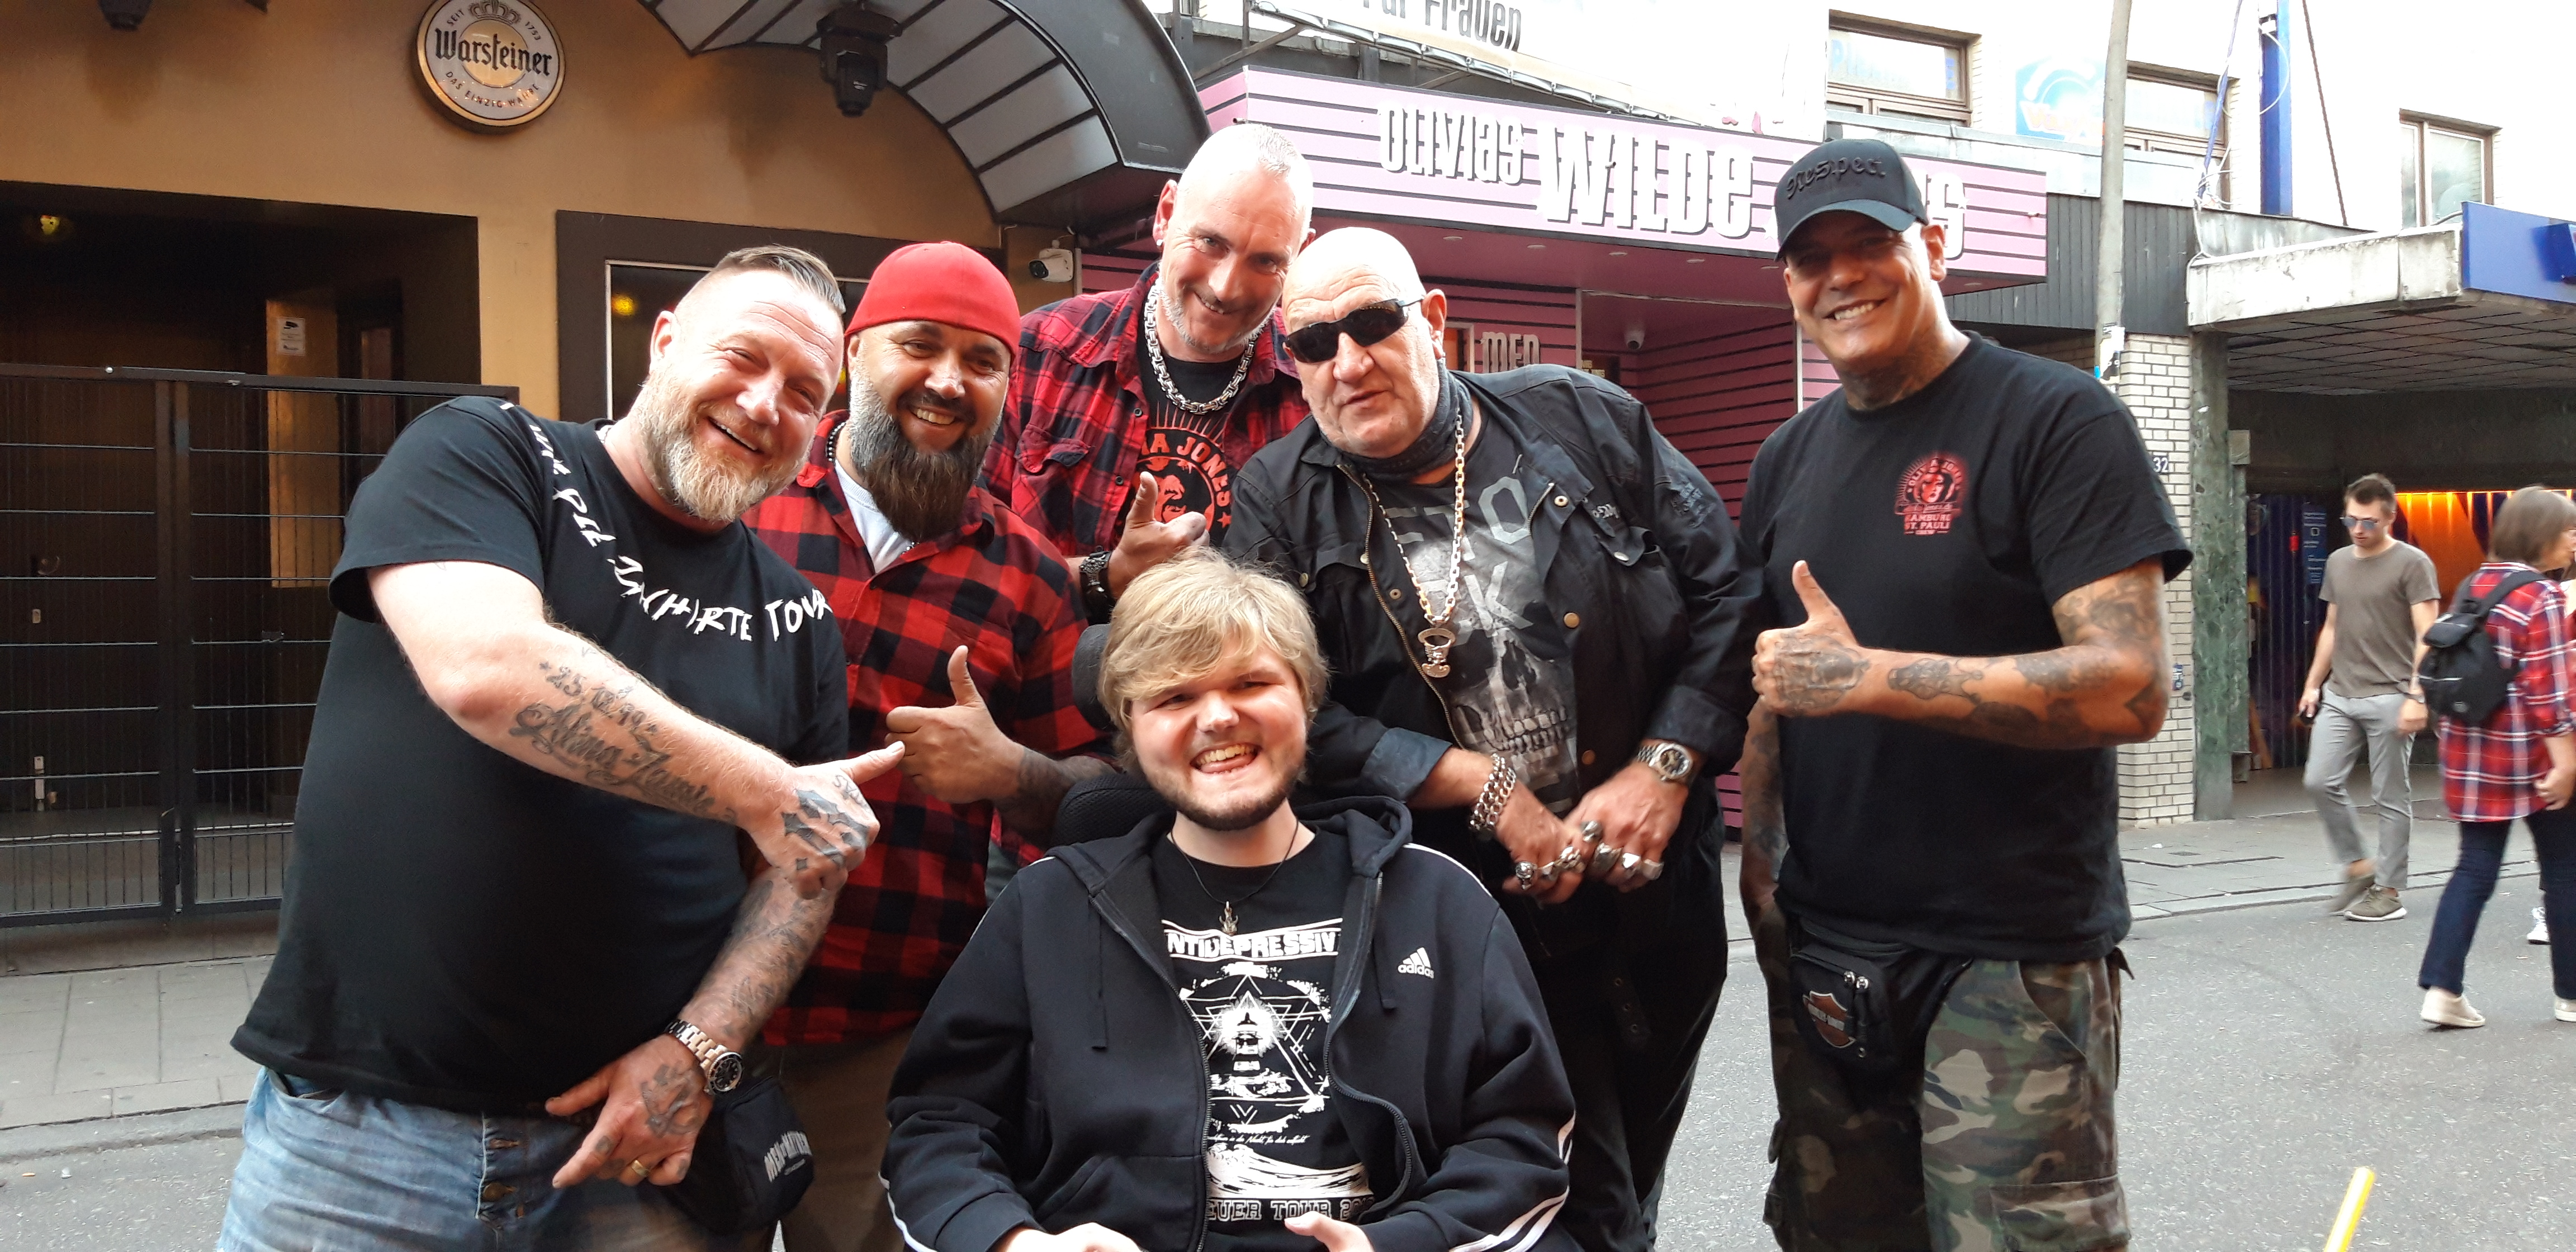
\includegraphics[width=\textwidth]{Fotos/kiez.jpg}}
    \caption{Fabian (links) und seine Kumpels von der Großen Freiheit. Ich hatte die Ehre, von ihm in einer Privattour über den Kiez geführt zu werden.}
    \label{fig:hamburg}
\end{figure}

Allerdings gibt es auch einen Wermutstropfen. Als Stadt am Wasser hat Hamburg auch mit Sturmfluten und Überschwemmungen zu rechnen. Die Eingänge vieler, vor allem älterer Häuser, befinden sich drei bis vier Stufen über Straßenniveau. Darunter sind auch viele Restaurants, die für Rollstuhlfahrer wie mich deshalb unerreichbar sind. Auch sind längst nicht alle Bordsteine abgesenkt, so dass man oft hunderte von Metern Umwege fahren muss, bis man eine Absenkung gefunden hat. Auch Hamburgs U-Bahn-Netz ist mit dem von München oder Berlin nicht zu vergleichen. In Hamburg fährt man als Rollstuhlfahrer:in besser mit dem Bus, wenn man größere Strecken zurücklegen muss.

\section{Berlin}

Last but not least ist da natürlich Berlin. Berlin ist speziell. Speziell aufgrund seiner Geschichte. Der Kalte Krieg, die ehemalige DDR und die Mauer sind in der Stadt allgegenwärtig. Berlin ist vielseitig. Ich habe bei meinen Aufenthalten drei der 12 Stadtbezirke näher kennen- und lieben gelernt. Jeder von ihnen hat einen ganz speziellen Charme.

Im Bezirk Mitte findet man die meisten und die bekanntesten Sehenswürdigkeiten: das Brandenburger Tor, den Fernsehturm, den Gendarmenmarkt – ein wunderschöner historischer Markplatz – und den Potsdamer Platz, ein wichtiger Verkehrsknotenpunkt mit einer Ansammlung moderner Gebäude, in denen sich viele gute Restaurants befinden.

Ein besonders bunter Bezirk ist Friedrichshain-Kreuzberg. Der Szene-Bezirk ist multikulturell geprägt und lockt mit Bars, Cafés und Trödelläden. Es gibt dort einiges zu entdecken, darunter die East Side Gallery, eine Open-Air-Galerie an dem längsten noch erhaltenen Teilstück der Berliner Mauer, oder das Mauermuseum am Checkpoint Charlie. An der Warschauer Brücke im Bezirk Friedrichshain-Kreuzberg befindet sich das RAW-Gelände, ein riesiges, 52.000 m2 großes Areal, dessen Eigentümer die Deutsche Bahn war (RAW steht für Reichsbahnausbesserungswerk). RAW ist ein alternatives Kulturprojekt mit vielen Clubs, Restaurants, Hallen zum Indoor-Klettern, einem Kulturzentrum und einem Flohmarkt, der jeden Sonntag stattfindet. Muss man gesehen haben.

Auch der Bezirk Neukölln hat sich in den letzten Jahren zu einem Szene-Stadtteil mit großer Kunst- und Kulturszene, vielen Galerien, Cafés und Kneipen entwickelt. Wer auf internationale Leckereien steht, wird hier fündig.

Was die Unterbringung angeht, kann ich das Hotel Grenzfall an der Ackerstraße, Ecke Bernauer Straße empfehlen. Es liegt in unmittelbarer Nähe zur Gedenkstätte Berliner Mauer, dem zentralen Erinnerungsort an die deutsche Teilung, der sich auf 1,4 km Länge entlang der Bernauer Straße über den ehemaligen Grenzstreifen erstreckt.

Das Hotel ist barrierefrei, alle Zimmer sind mit dem Aufzug erreichbar. Die 16 sogenannten Klassikzimmer sind 20 m2 groß und verfügen über eine bodenebene Dusche. Vier dieser Zimmer sind speziell an den Bedürfnissen von Rollstuhlfahrer:innen ausgerichtet und entsprechen der DIN 18025-1. Das Bad ist bei ihnen deutlich größer als bei den anderen Zimmern.

Das Berliner U-Bahn- und S-Bahn-Netz ist ein Traum. Aufzüge für Rollstuhlfahrer gibt es gefühlt an jeder zweiten Straßenecke. Was ich wärmstens empfehlen kann, ist übrigens die Anschaffung einer leichten, robusten und faltbaren Rampe aus Kohlefaser, die man an den Rollstuhl hängen kann, um Hindernisse zu überbrücken, wie beispielsweise den Spalt zwischen Bahnsteig und Waggon. Zugegebenermaßen sie sind nicht ganz billig, aber für einen Stadturlaub eigentlich unerlässlich.

\section{New York}

Um es gleich vorwegzunehmen: an New York kommt – mit großem Abstand – keine Stadt heran, zumindest keine, die ich kenne (zugegebenermaßen sind das nicht so viele). New York ist anders, unvergleichlich, eine andere Welt. Ich wollte unbedingt einmal im Leben dorthin. Im August 2011, während der Sommerferien, war es soweit. Wir flogen nach Big Apple!

Mit den Planungsvorbereitungen hatten meine Eltern bereits ein Jahr zuvor begonnen. Mit einem Sohn, der in einem 150 kg schweren, sperrigen E-Rollstuhl sitzt, fliegt man nicht mal eben Last Minute über den Atlantik, wie ihr euch sicherlich vorstellen könnt. Die Logistik dieser Reise war eine echte Herausforderung. Das begann schon mit der Frage, wann wir fliegen würden. Eigentlich ist der August für einen Urlaub in New York nicht der ideale Monat. Tagsüber erreichen die Temperaturen dort locker 30° Celsius und mehr. Entweder steht die Luft an Tagen mit wenig Wind und – als sei das nicht genug – die Wolkenkratzer strahlen zusätzlich noch eine unerträgliche Hitze ab, oder aber es weht ein heißer Fön-artiger Wind durch die Straßenschluchten, was auch nicht besser ist. Wem Hitze nichts ausmacht und sie vielleicht sogar mag, der wird im August nicht enttäuscht werden. Wer es lieber ein wenig kühler aber immer noch warm haben möchte, der sollte im Juni nach New York reisen.

Tatsächlich war ich in beiden Monaten schon einmal in New York, einmal im August 2011 und dann noch einmal im Juni 2013. Ich werde euch hier ein wenig von meinen gesammelten Erfahrungen während dieser beiden jeweils 10-tägigen Aufenthalte in New York erzählen.

Die erste Frage, die sich meinen Eltern stellte, betraf den Abflug- sowie den Zielflughafen. 2011 konnte man entweder Nonstop von Düsseldorf nach Newark fliegen oder aber von Frankfurt nach John F. Kennedy International Airport, kurz JFK. Da wir nur knapp 30 km vom Düsseldorfer Flughafen entfernt wohnen, bot es sich natürlich an, von dort zu fliegen und sich den zusätzlichen Aufwand einer mindestens zweistündigen Autofahrt nach Frankfurt zu ersparen.

Die Strecke Düsseldorf-Newark hat aber gegenüber der Strecke Frankfurt-JFK noch einen anderen, entscheidenden Vorteil. Obwohl der Flughafen Newark nicht im Bundesstaat New York liegt, sondern im südlich angrenzenden Nachbarstaat New Jersey, ist es viel einfacher, von dort aus nach Manhattan zu kommen als von JFK aus, der am entfernten Ende der Insel Long Island liegt und eine Fahrt durch den riesigen Stadtteil Brooklyn erfordert, um nach Manhattan zu gelangen.

Newark liegt von Manhattan aus gesehen Luftlinie etwa 16 km entfernt auf der anderen Seite des Hudson Rivers (wo der Pilot Chesley Sullenberger im Januar 2009 einen Airbus der Airline US Airways nach Ausfall beider Triebwerke in einer fliegerischen Meisterleistung notgewassert und alle 150 Passagiere gerettet hat). Von dort aus gelangt man mit dem Amtrak-Zug innerhalb von nur 45 Minuten direkt ins Herz von Manhattan, zum Bahnhof Penn Station, der unterhalb der runden Madison Square Garden Veranstaltungshalle in Midtown an der Ecke 8. Avenue, 33. Straße liegt. Einfacher geht’s nicht.

Klugerweise hatten meine Eltern ein Zimmer in einem Hotel gebucht, das in unmittelbarer Nähe zur Penn Station liegt und über mehrere geräumige Doppelzimmer für Rollstuhlfahrer:innen mit Begleitung verfügt. Das New Yorker Hotel befindet sich an der Ecke 8. Avenue, 34. Straße, in einer Sichtlinie mit dem Empire State Building und keine 800 m von diesem entfernt. Ein wirklich tolles Hotel, in unschlagbarer Lage.

Doch nochmal zurück zum Flug. Es ging also von Düsseldorf aus nach New York. Beim Planen des Fluges hatten sich meine Eltern mit dem Mobilitätsservice der Lufthansa in Verbindung gesetzt, um sich darüber zu informieren, was bei einer Reise mit E-Rollstuhl so alles zu beachten ist. Vor allem ging es um die Fragen, wie mein E-Rollstuhl in den Frachtraum gelangt, auf welchem Rollstuhl ich in der Zwischenzeit Platz nehme und wie ich zu guter Letzt ins Flugzeug komme.

Wir mussten den Rollstuhl drei Stunden vor Abflug als Sperrgepäck abgeben. Nachdem man mich auf einen Ersatzrollstuhl umgesetzt hatte, wurde mein Permobil C500 gründlich untersucht und durchleuchtet. Ganz wichtig ist es, Werkzeug dabei zu haben, um die beiden Batterien vom Stromkreislauf des Rollstuhls abzuklemmen.

Wir passierten anschließend die Security und gingen dann in Richtung Gate. Geschoben wurde ich von einem Flughafen-Mitarbeiter. Am Gate mussten wir dann eine Stunde warten, bis das Boarding losging. Ich war der erste, der an Board ging. Ich wurde erneut umgesetzt, und zwar diesmal auf einen sehr schmalen Kabinenrollstuhl, der gerade so breit war, dass er durch den schmalen Gang zwischen den Sitzreihen des Fliegers passte. Mit ihm wurde ich an meinen Sitzplatz gerollt und dort von meinen Eltern auf einen der für uns reservierten Sitzplätze umgesetzt. Der Mobilitätsservice hatte dafür gesorgt, dass wir eine Sitzreihe unmittelbar hinter einer Trennwand hatten. Diese hatte etwas mehr Beinfreiheit, so dass es für meine Eltern etwas leichter war, wenn sie mir halfen.

Der Flug dauerte gut 10 Stunden und verlief bis auf die Tatsache, dass ich einmal pinkeln musste (die Stewardessen halfen, indem sie einen Vorhang hielten, um mich vor den Blicken anderer Passagiere zu schützen), unspektakulär. Trotzdem tat mir der Hintern weh. In Newark angekommen wurde ich mit dem Kabinenrollstuhl diesmal als letzter Passagier aus dem Flugzeug gerollt. Man setzte mich wieder in einen Behelfsrollstuhl und zeigte uns, wo wir unser Gepäck und meinen E-Rollstuhl entgegennehmen konnten.

Meine Eltern und ich beteten, dass dieser während des Fluges nicht beschädigt wurde und wir schlimmstenfalls direkt unsere Rückreise hätten antreten müssen. Wer repariert in New York schon einen Permobil C500, bei dem beispielsweise während des Fluges im Frachtraum die elektronische Steuerung abgebrochen war. Und wie sollten wir zu einem Reparaturservice z.~B mitten in Brooklyn gelangen, falls es denn einen solchen überhaupt gibt und er über das passende Ersatzteil verfügt? Mit solchen Gedanken beschäftigte sich mein Vater den ganzen Flug über. Zum Glück hatte der Rollstuhl den Flug jedoch unbeschadet überstanden und wir machten uns nach Passieren der Security mit unserem Gepäck in Richtung Bahnhof auf. Einer unserer Koffer beinhaltete übrigens einen zerlegbaren Duschrollstuhl, einen solchen stellte das Hotel nämlich nicht zur Verfügung.

Nach einer zwanzigminütigen Fahrt mit einem Airtrain erreichten wird den Amtrak-Bahnhof, kauften die Tickets für die Fahrt nach New York und gingen zum Bahnsteig, wo wir an einer speziell gekennzeichneten Stelle für Rollstuhlfahrer:innen auf den Zug warteten. Als dieser schließlich einfuhr und hielt, stieg ein Schaffner aus und stellte eine Rampe auf, über die ich in den Waggon rollte. 40 Minuten später waren wir in Manhattan.

Ich vergesse niemals den Moment, als wir aus der Penn Station auf die Straße traten. Es war heiß und um den Himmel zu sehen, mussten wir unsere Köpfe in den Nacken legen und senkrecht nach oben schauen. Wir standen vor einem Wolkenkratzer, der nicht nur hoch, sondern auch breit war und den Großteil unseres Gesichtsfeldes bedeckte. So etwas hatten wir drei nicht nur noch nie gesehen, sondern es uns so gewaltig auch nicht vorgestellt. Nachdem unsere freudige Erregung abgeklungen war, machten wir uns in Richtung Hotel auf, das keine 5 Minuten Fußweg entfernt auf uns wartete.

Ich weiß nicht, wie viele Kilometer meine Eltern und ich in den 10 Tagen, die wir in New York waren, zu Fuß bzw. im Rollstuhl zurückgelegt haben, aber es waren etliche. Alleine zweimal sind wir von der südlichen Spitze Manhattans, dort, wo die Fähre nach Staten Island und zur Freiheitstatue ablegt, bis nach Midtown marschiert bzw. gefahren, um den Stadtteil Manhattan sozusagen der halben Länge nach kennenzulernen (und das auch nur entlang einer Avenue). Das geht nicht nur in die Beine, sondern auch auf die Batterie. Apropos Batterie: Spannungsumwandler für das Ladegerät und Steckdosen-Adapter nicht vergessen!

Dass New York den Spitznamen „The City that never sleeps“ trägt, kann ich gut nachvollziehen. Selbst nachts um 3 Uhr ging mindestens einmal pro Minute irgendwo in der Nähe die Sirene eines Polizei-, Feuerwehr- oder Krankenwagens.

Was mich an New York wirklich am meisten erstaunt hat, ist die Tatsache, dass man sofort zum New Yorker wird, sobald man aus dem Hotel kommt und auf die Straße geht. In New York laufen so viele Menschen unterschiedlichster Ethnien rum, dass man als Tourist sofort in der Menge aufgeht, mit ihr verschmilzt und von anderen für einen New Yorker gehalten wird.

Erstaunlich ist auch, wie leicht man sich in New York zurechtfindet. Manhattan ist in die drei Abschnitte Downtown, Midtown und Uptown unterteilt. Downtown liegt südlich vom Union Square. Midtown beginnt nördlich davon und reicht bis zur 59th Straße. Uptown ist alles nördlich der 59th Straße, etwa ab Höhe Central Park. Die Straßen sind nach einem Gittersystem angelegt. Straßen (Streets) verlaufen waagerecht von Ost nach West und Alleen (Avenues) senkrecht von Nord nach Süd. Die Fifth Avenue teilt New York in West (W) und Ost (E). Das Gebäude 150 E 34th liegt also östlich Fifth Avenue auf der 34. Straße und hat die Hausnummer 150.

\setlength{\fboxsep}{0pt}    % Kein Abstand zwischen Rahmen und Bild
\setlength{\fboxrule}{0.2pt} % Rahmenstärke auf 0.2 pt setzen
\begin{figure}[ht]
    \raggedright
    \fcolorbox{rahmenlinie}{white}{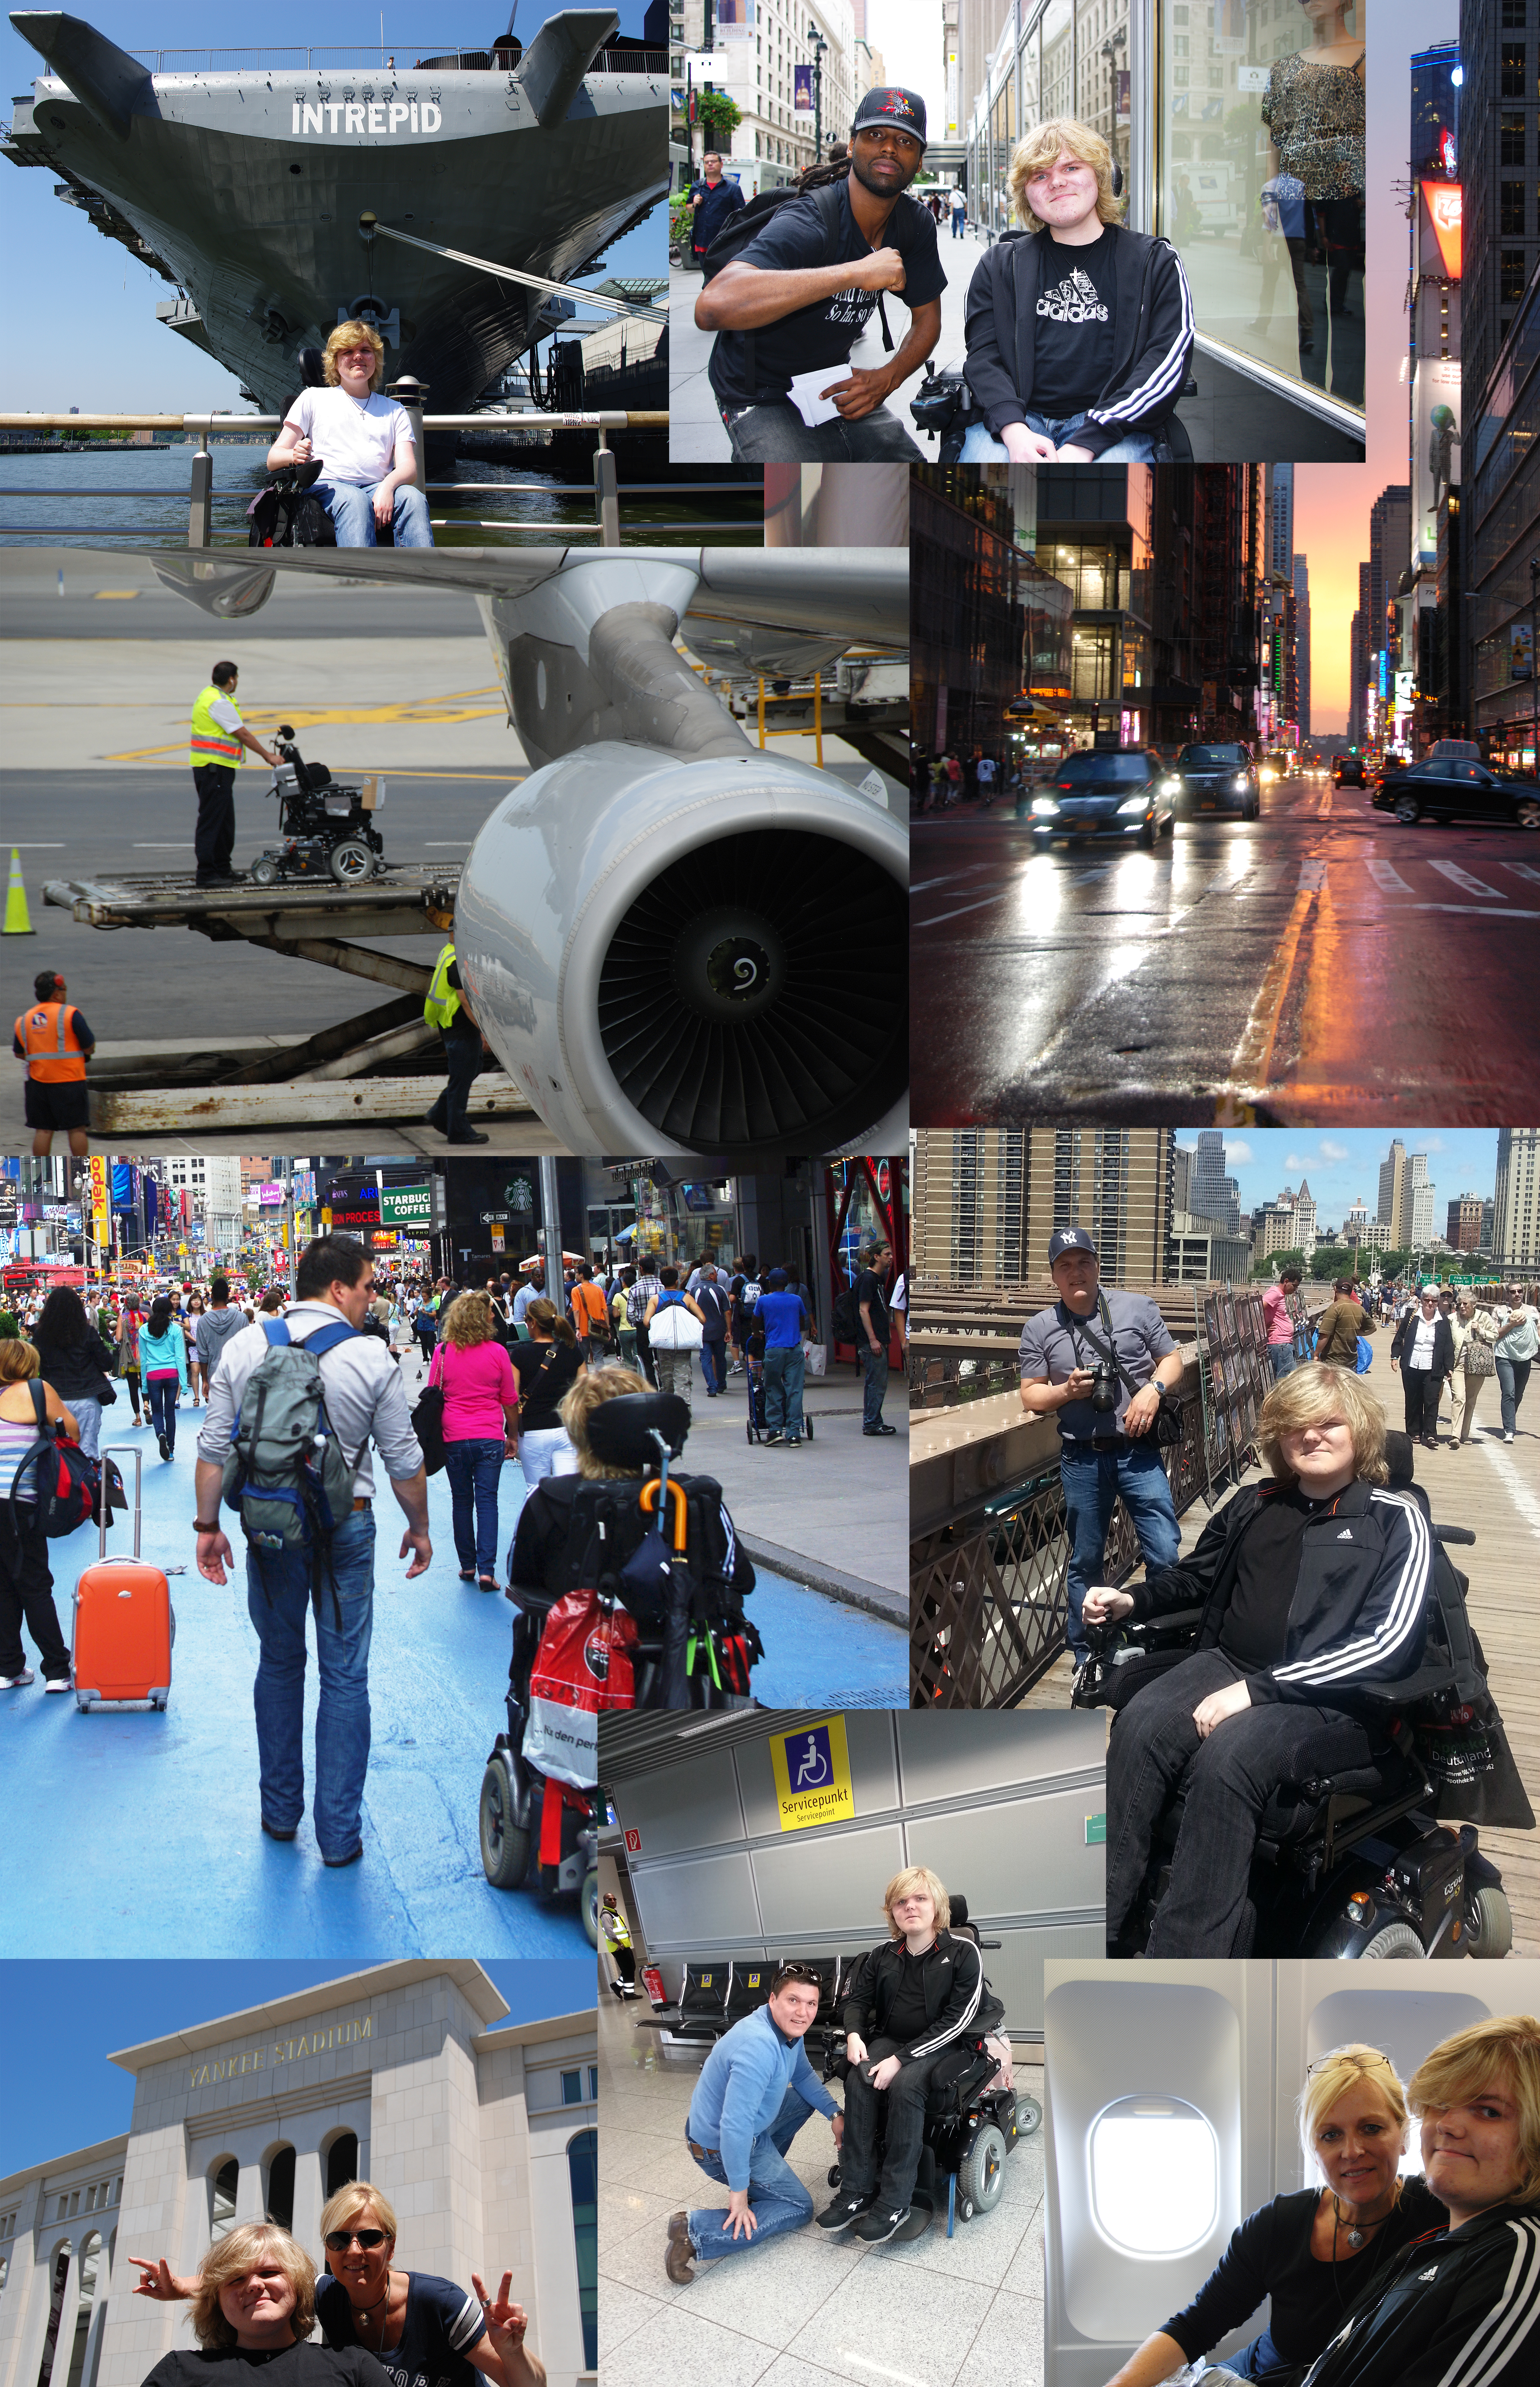
\includegraphics[width=\textwidth]{Fotos/New York Collection.jpg}}
    \caption{Es gibt so viel zu sehen und zu erleben in New York. Hier ein paar Eindrücke von meinen Aufenthalten in der Stadt, die niemals schläft.}
    \label{fig:new_york_collection}
\end{figure}

\end{document}
